%%%%%%%%%%%%%%%%%%%%%%%%%%
% USFD Academic Report Template
% Prof. Roger K. Moore
% University of Sheffield
% 30 July 2018
%%%%%%%%%%%%%%%%%%%%%%%%%%


\documentclass[11pt,oneside]{book}
\usepackage[margin=1.2in]{geometry}
\usepackage[toc,page]{appendix}
\usepackage{amssymb}
\usepackage{amstext}
\usepackage{amsmath}
\usepackage{amsthm}
\usepackage{dirtytalk}
\usepackage{graphicx}
% \usepackage{natbib}
\usepackage[square,numbers]{natbib}
\usepackage{lipsum}
\usepackage{caption}
\usepackage{subcaption}

%
\usepackage{mathtools}
\usepackage{fontawesome}
%

\usepackage{xcolor}


\newtheorem{theorem}{Theorem}
\renewcommand*{\thefootnote}{\fnsymbol{footnote}}

\begin{document}

\captionsetup[figure]{margin=1.5cm,font=small,labelfont={bf},name={Figure},labelsep=colon,textfont={it}}
\captionsetup[table]{margin=1.5cm,font=small,labelfont={bf},name={Table},labelsep=colon,textfont={it}}
\setlipsumdefault{1}

\frontmatter

\begin{titlepage}


% -------------------------------------------------------------------
% You need to edit the details here
% -------------------------------------------------------------------

% [ML based Outlier Detection for DC]{Machine Learning Based Outlier Detection for Data Certification}

\begin{center}
{\LARGE CERN Summer Student Report 2019}\\[1.5cm]
\linespread{1.2}\huge {\bfseries Machine Learning Based Outlier Detection for Data Certification}\\[1.5cm]
\linespread{1}
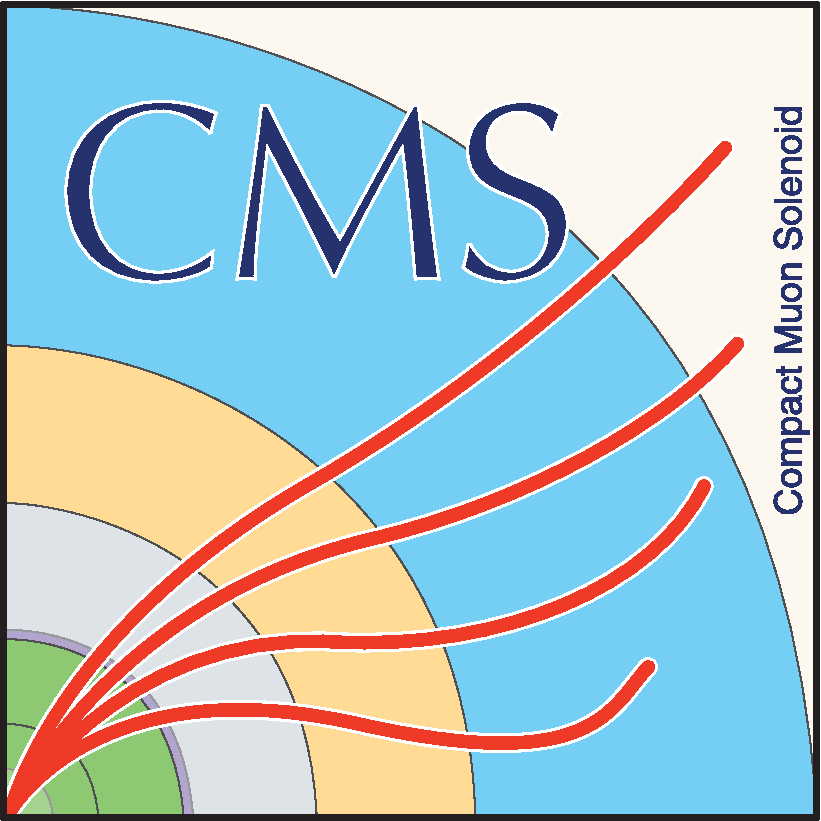
\includegraphics[width=3cm]{images/CMS_logo_May2014-eps-converted-to.pdf}\\[1cm]
{\Large Patomporn Payoungkhamdee \footnote{Mahidol University} \\ EP-CMG-CO}\\[1cm]
{\large \emph{Supervisor:} Marcel Andre Schneider \footnote{European Organization for Nuclear Research (CERN)}}\\[1cm]
% {\large \emph{Supervisor:} Marcel Andre \say{The Lightning \text{\faBolt}} Schneider \footnote{European Organization for Nuclear Research (CERN)}}\\[1cm]
\large A report submitted in partial fulfilment of the requirements\\ for the CERN summer student programme 2019 \\[2cm] 
August 22, 2019
\end{center}

\end{titlepage}


% -------------------------------------------------------------------
% Declaration
% -------------------------------------------------------------------

% \newpage
% \section*{\Large Declaration}

% All sentences or passages quoted in this document from other people's work have been specifically acknowledged by clear cross-referencing to author, work and page(s).  Any illustrations that are not the work of the author of this report have been used with the explicit permission of the originator and are specifically acknowledged.  I understand that failure to do this amounts to plagiarism and will be considered grounds for failure.\\[1cm]

% \noindent Name:\\[1mm]
% \rule[1em]{25em}{0.5pt}

% \noindent Signature:\\[1mm]
% \rule[1em]{25em}{0.5pt}

% \noindent Date:\\[1mm]
% \rule[1em]{25em}{0.5pt}


% -------------------------------------------------------------------
% Abstract
% -------------------------------------------------------------------

\chapter*{\Large \center Abstract}

% Guidance of how to write an abstract/summary provided by Nature: https://cbs.umn.edu/sites/cbs.umn.edu/files/public/downloads/Annotated_Nature_abstract.pdf

Compact Muon Solenoid (CMS) detector was built in the middle of collision from LargeHadron Collider (LHC) which is one of the most powerful particle accelerators in the world. The mission is to collect the product from collision and decaying which happens 40 million times each second. The data taking in the CMS experiment is reconstructed to become a physics quantity 48 hours after a collision. The certification of data quality is made on run and lumisection levels. The criteria to certify are both from an automatic system as well as manual work from untraceable misbehaving of detector which is marked by offline shifter and detector experts. Approximately 95\% of data are good and the rest of them are bad. It is not easy to say that all phenomena that cause misbehaving of a result are well understood. Then the aim of this work is to reduce the manual work for data qualification by exploding various types of semi-supervised learning by treating the outlier as bad in lumisection granularity.
\chapter*{Acknowledgement}


\begin{itemize}
    \item CERN Summer Student program 2019
    \item Especially
    \begin{itemize}
        \item Marcel Andre Schneider
        \item Francesco Fiori
        \item Kaori Maeshima
        \item Adrian Alan Pol
        \item Countless CMS DQM people
    \end{itemize}
    \item GPU resources from IBM in collaboration with CERN Openlab
\end{itemize}


% \begin{minipage}{0.8\textwidth}
% \end{minipage}\hfill
% \begin{minipage}{0.1\textwidth}
%     
\includegraphics[width=\linewidth,keepaspectratio]{images/ibm.png}
% \end{minipage}\hfill
% \begin{minipage}{0.1\textwidth}
%     
\includegraphics[width=\linewidth,keepaspectratio]{images/cern_openlab.png}
% \end{minipage}

\begin{figure}[h!]
    \begin{subfigure}[b]{1.2in}
        
\includegraphics[width=\linewidth]{images/ibm.png}
    \end{subfigure}
    \begin{subfigure}[b]{1.8in}
        
\includegraphics[width=\linewidth]{images/cern_openlab.png}
    \end{subfigure}
\end{figure}


% -------------------------------------------------------------------
% Contents, list of figures, list of tables
% -------------------------------------------------------------------

\tableofcontents
\listoffigures
% \listoftables


% -------------------------------------------------------------------
% Main sections (as required)
% -------------------------------------------------------------------

\mainmatter

\chapter{Overview}

Before the whole data be feeding to physics analysis, there are a procedure to certify the data quality in run and lumisection granularity.
Data quality monitoring (DQM) team provide the tools and workflow where there are offline and online section to consider which basically online is a real time and the data that we get 2 days after collision would be inspected in offline section.
There are the person who looking at a dozen of histogram that demenstrate the occupancy of detector in each sub-system and also the physics quantities in various perspective of information.
Most of Bad lumisection (LS) are automatically came from run tagged as bad by human for the whole run and DCS bits in lumisection levels. In some cases, there are a small fraction bad LS that are manually marked as bad by data certification experts in lumisection levels because some kind of detector malfunction isn't tracable from the previous process.
On the other hand, good LS are defined in Golden JSON which are literally taken from data that passes of of those bad criteria.

The main objective of this work is to find a mathematical way to certify data quality in lumisection granularity to reduce the mannual work of data certification experts.
As you might have seen that there are only a small fraction of data. Moreover, the bad data that are marked by the expert are relatively small compare to a good data.
Then we have to face to the imbalance class problem and it is the reason why we choosing semi-supervised learing where we feed only good data to train the unsupervise model and testing with both kind of data.
Consequenly, the data that are mark as bad by the model would be consider as outlier where model does not familier with. The more explicit analysis would be provided in this report.
\chapter{Background}

%%%%%%%%%%%%%%%%%%%%%%
%        CMS
%%%%%%%%%%%%%%%%%%%%%%

\section{Compact Muon Solenoid (CMS) Detector}

The Compact Muon Solenoid (CMS) detector be designed for collect the collision and decaying data in forward and transverse of the beamline.
It has more resolution in the transverse direction from the equipment that has been designed to focus in transverse direction as the Figure \ref{fig:cms_structure}.
According to \cite{cms_design_report}, The detector itself consist of different sub-detector for their own purpose where the main components are
\begin{figure}[h!]
    \centering
    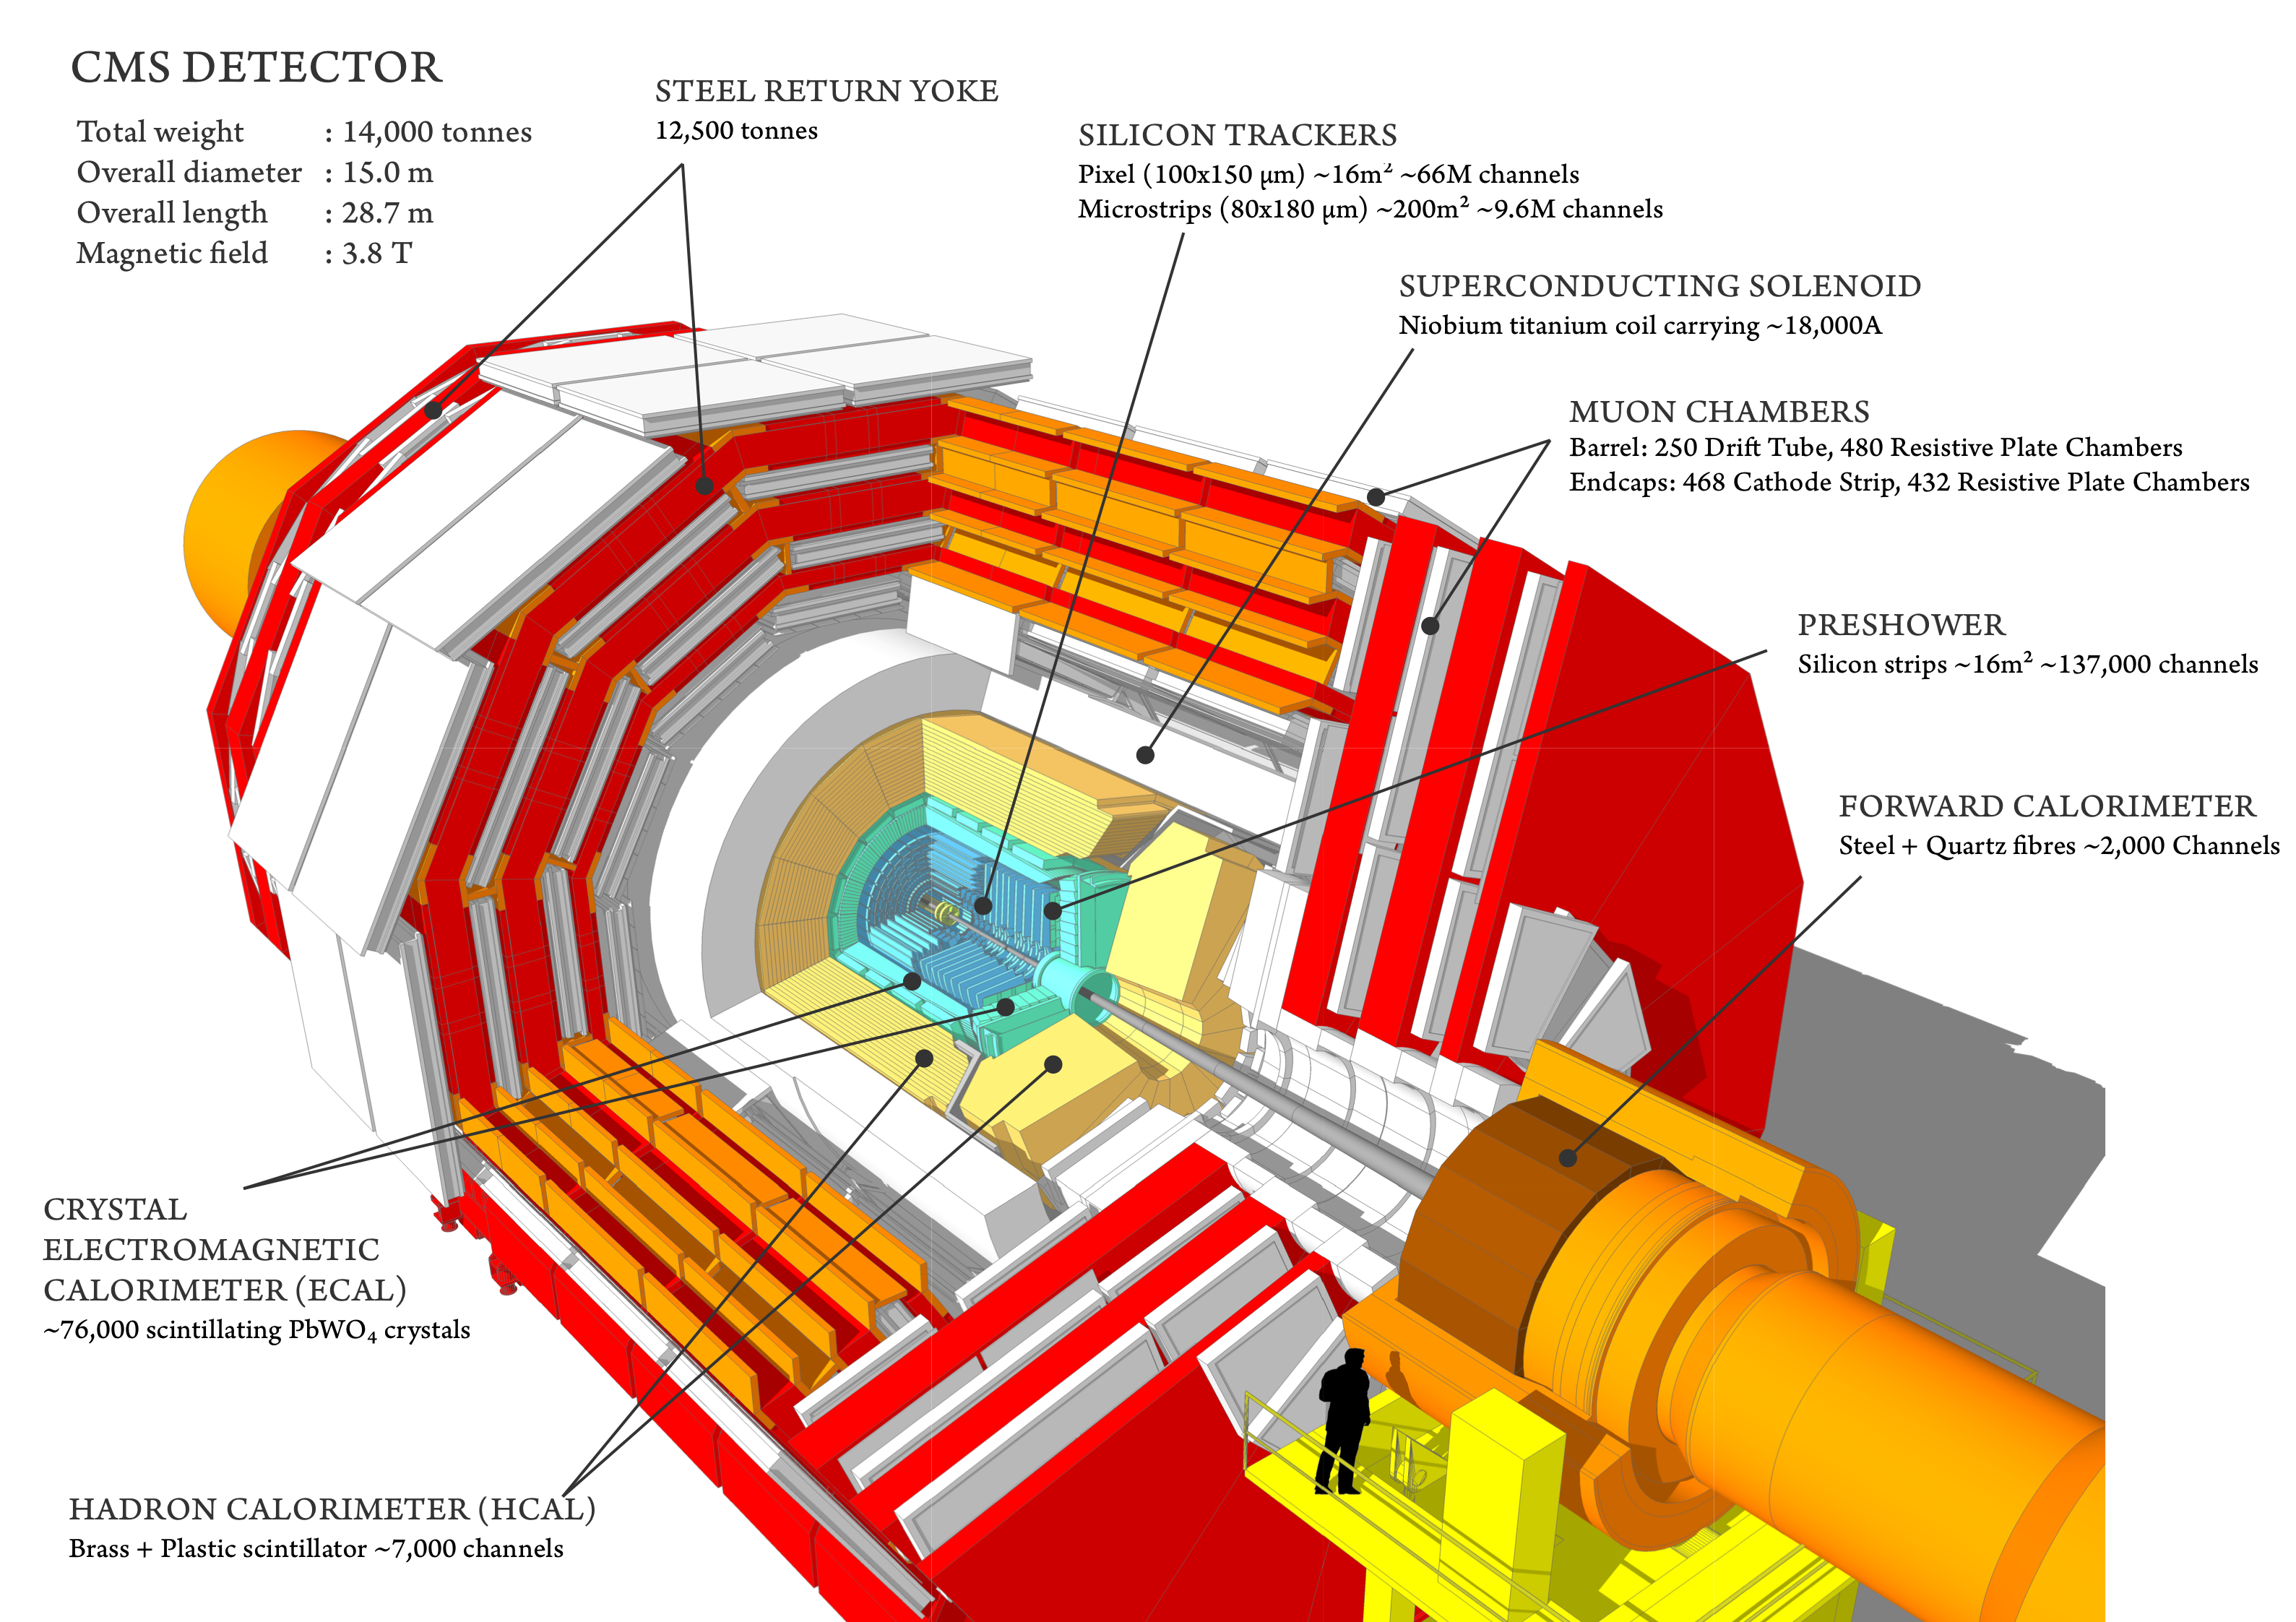
\includegraphics[width=0.8\textwidth]{images/cms_structure.png}
    \caption{Sectional view of the CMS detector. The LHC beams travel in opposite directions along the central axis of the CMS cylinder colliding in the middle of the CMS detector. Image retrieved from http://cms.web.cern.ch/news/cms-detector-design}
    \label{fig:cms_structure}
\end{figure}
\begin{enumerate}
    \item \textbf{Tracker} to trace the footprint of charge particle by beginning at the hitting of the closest layer which is pixel detector and following by multiple layer of strip detector to gain more precision of particle track that are correspond to momentum of the particle
    \item \textbf{Electromagnetic Calorimeter (ECAL)} measure the momentum of leptons (especially electron) and photon where the main interaction obviously is electromagnetic interaction
    \item \textbf{Hadron Calorimeter (HCAL)} has been designed for measure the energy of haronic particle where it also has QCD interaction rather than only electromagnatic
    \item \textbf{Superconducting Solenoid} for generate a nearly-uniform magnetic field inside of the cylindrical shape and definitely charge particle turn their heading around where it propagate in the outside of this radius like a muon track in Figure \ref{fig:cms_slide}
    \item \textbf{Muon Detectors} is one of the most important sub-detector for measuring the muon momentum and the track of them by also take the footprint tracking system into account to get more precise information which is also the most important task of CMS detector
\end{enumerate}
\begin{figure}[h!]
    \centering
    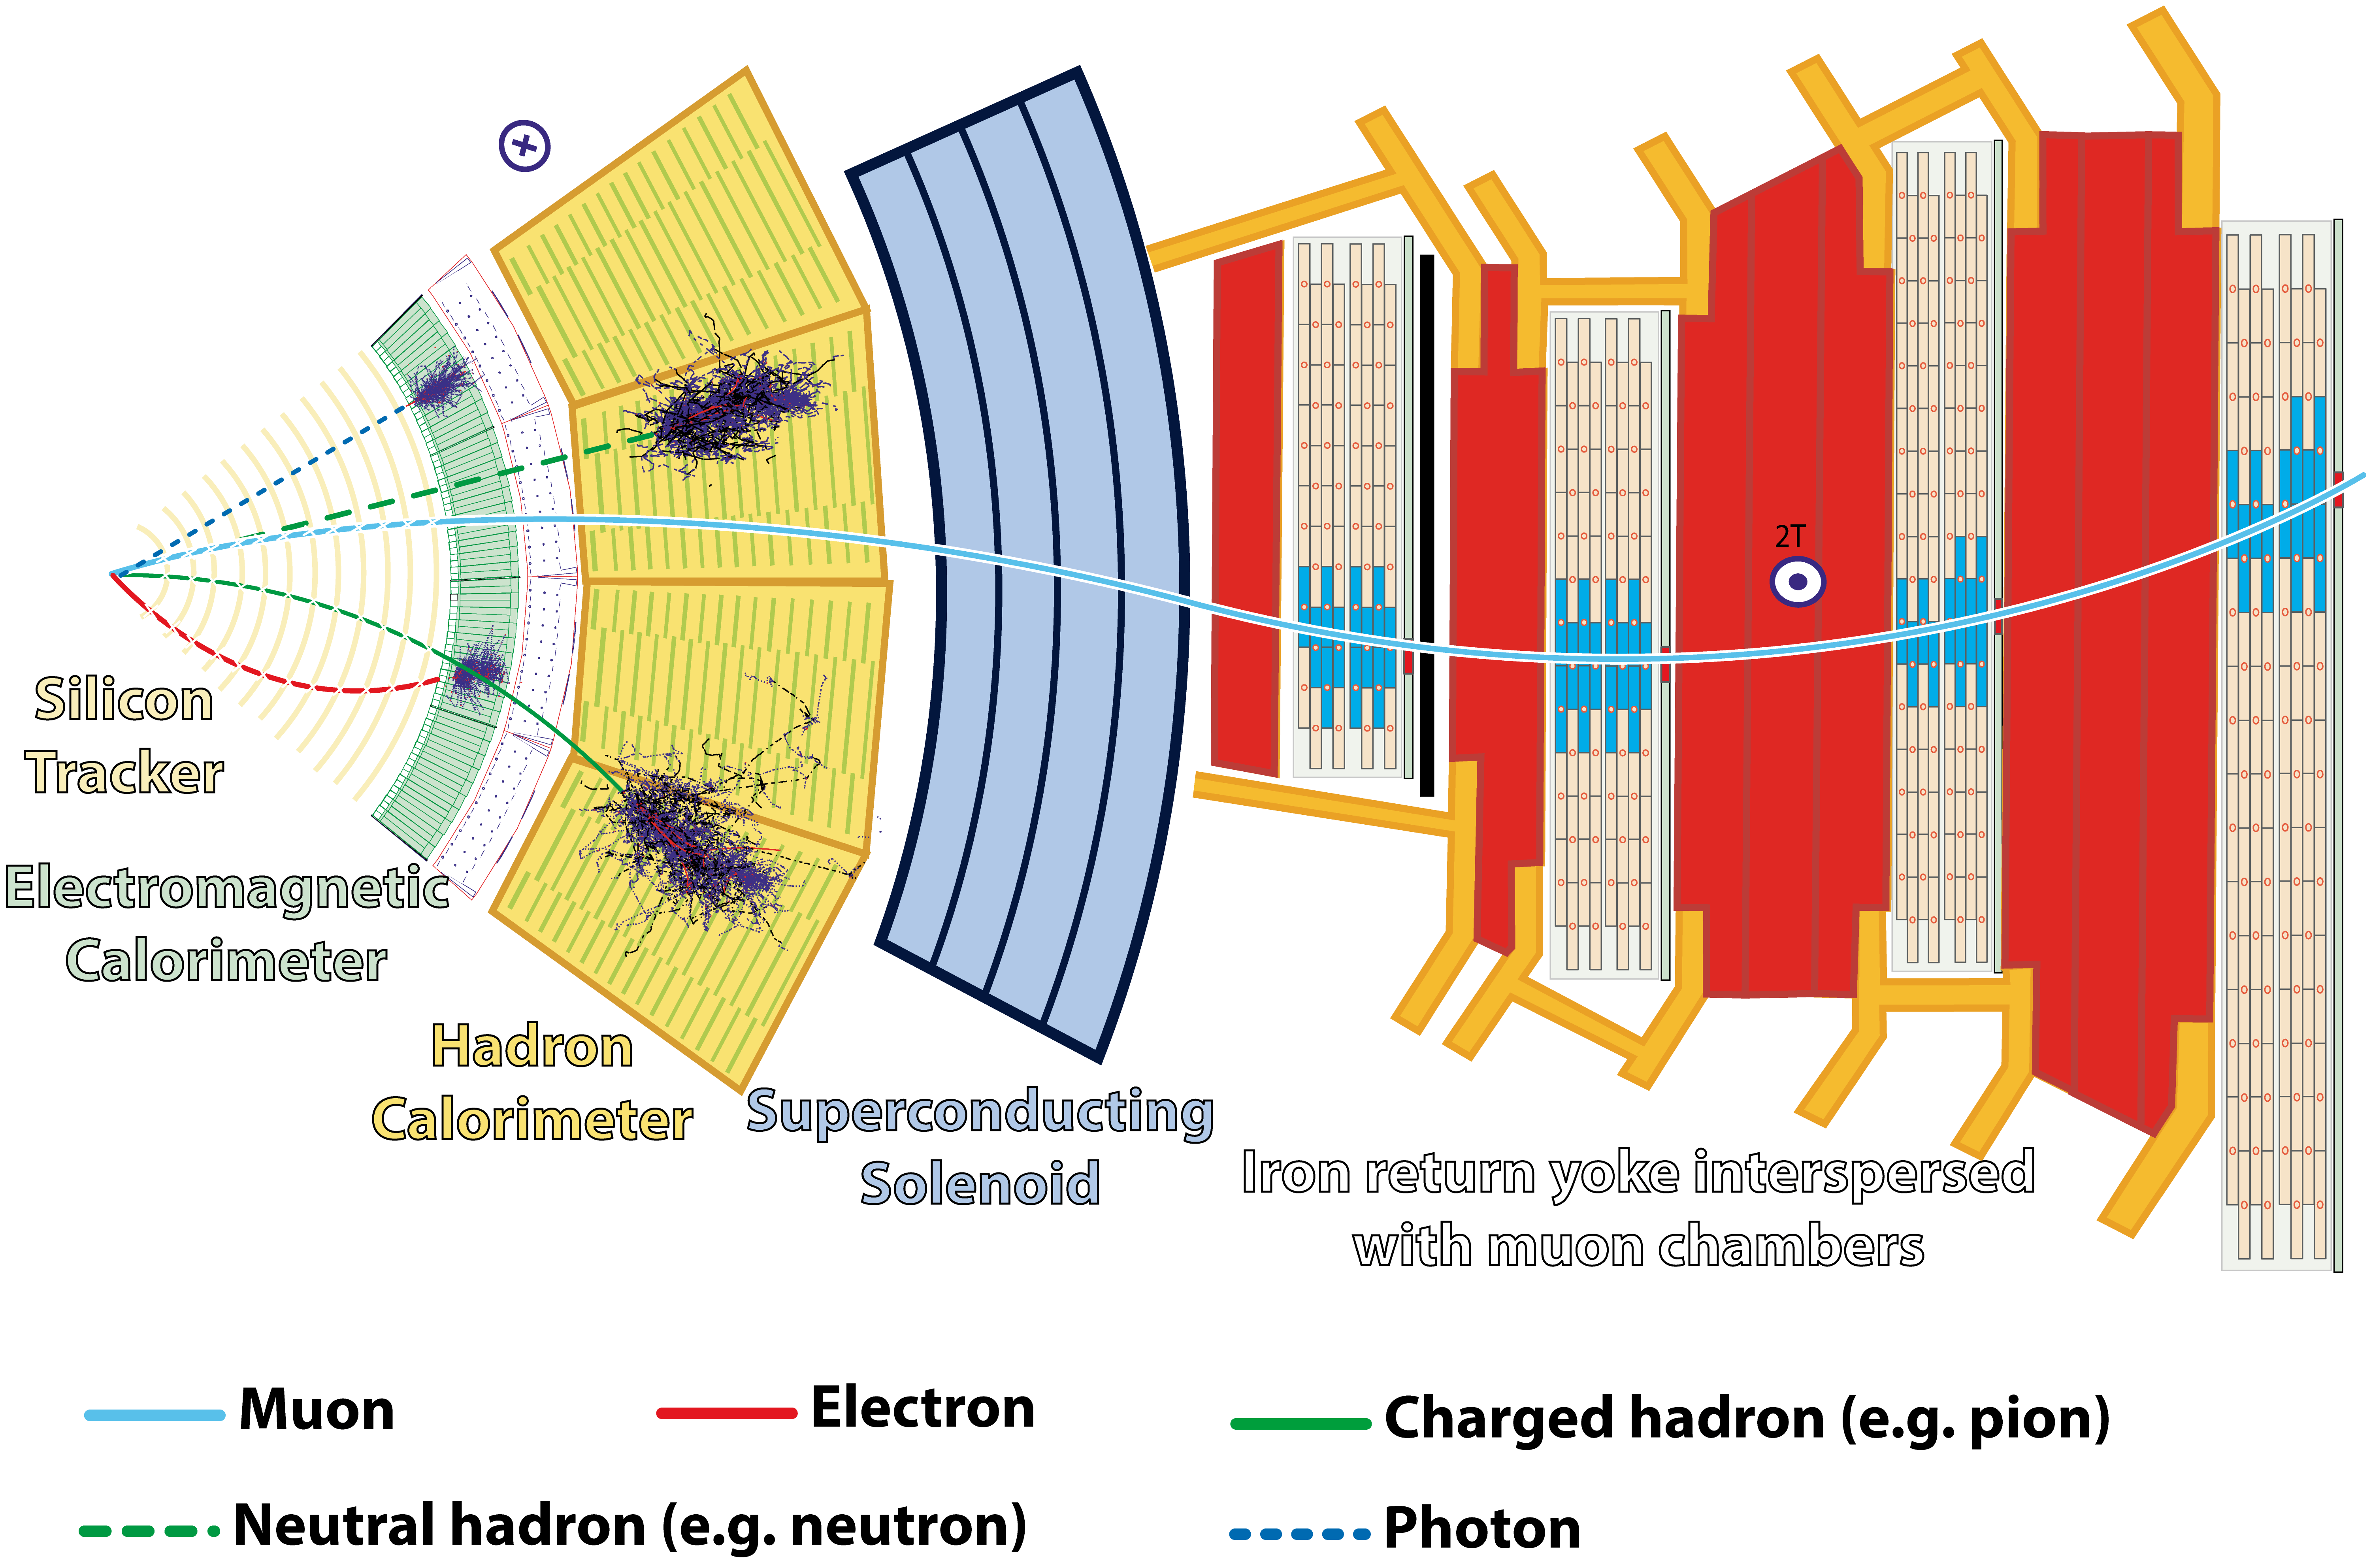
\includegraphics[width=0.8\textwidth]{images/cms_slide.png}
    \caption{Onion-like crossection of CMS. Image retrieved from \cite{cms_onion}}
    \label{fig:cms_slide}
\end{figure}


%%%%%%%%%%%%%%%%%%%%%%
%     CMS-DAQ
%%%%%%%%%%%%%%%%%%%%%%

\section{Data Acquisition (DAQ)}


According to \cite{cms_tridas_2002}, the collision rate takes around 40Mhz (100 Tbyte/s) which is impossible for the instrument to ollect all of those signal that happen at a time.
The harvested signal that CMS detector select are determined from low level trigger where the detector frontend (electronic circuit determination) process to select an interesting signal.
The level-1 (L1) trigger filter and produce the signal at 100 kHz (100 Gbyte/s). Then it has been send to high level trigger (HLT) where we could start to really see the interpretable physical quantities from here.

\subsection{CMS Online System}

CMS team also provide the tools for automate data acquisition as \cite{cms_daq} where the big picture has been demonstrated in Figure \ref{fig:cms_online_system}.
Apparently, the system still need some people to double check by using various tools e.g. Web GUI and so on during the running process of beam collider in LHC from the low level system to high level system.
\begin{figure}[h!]
    \centering
    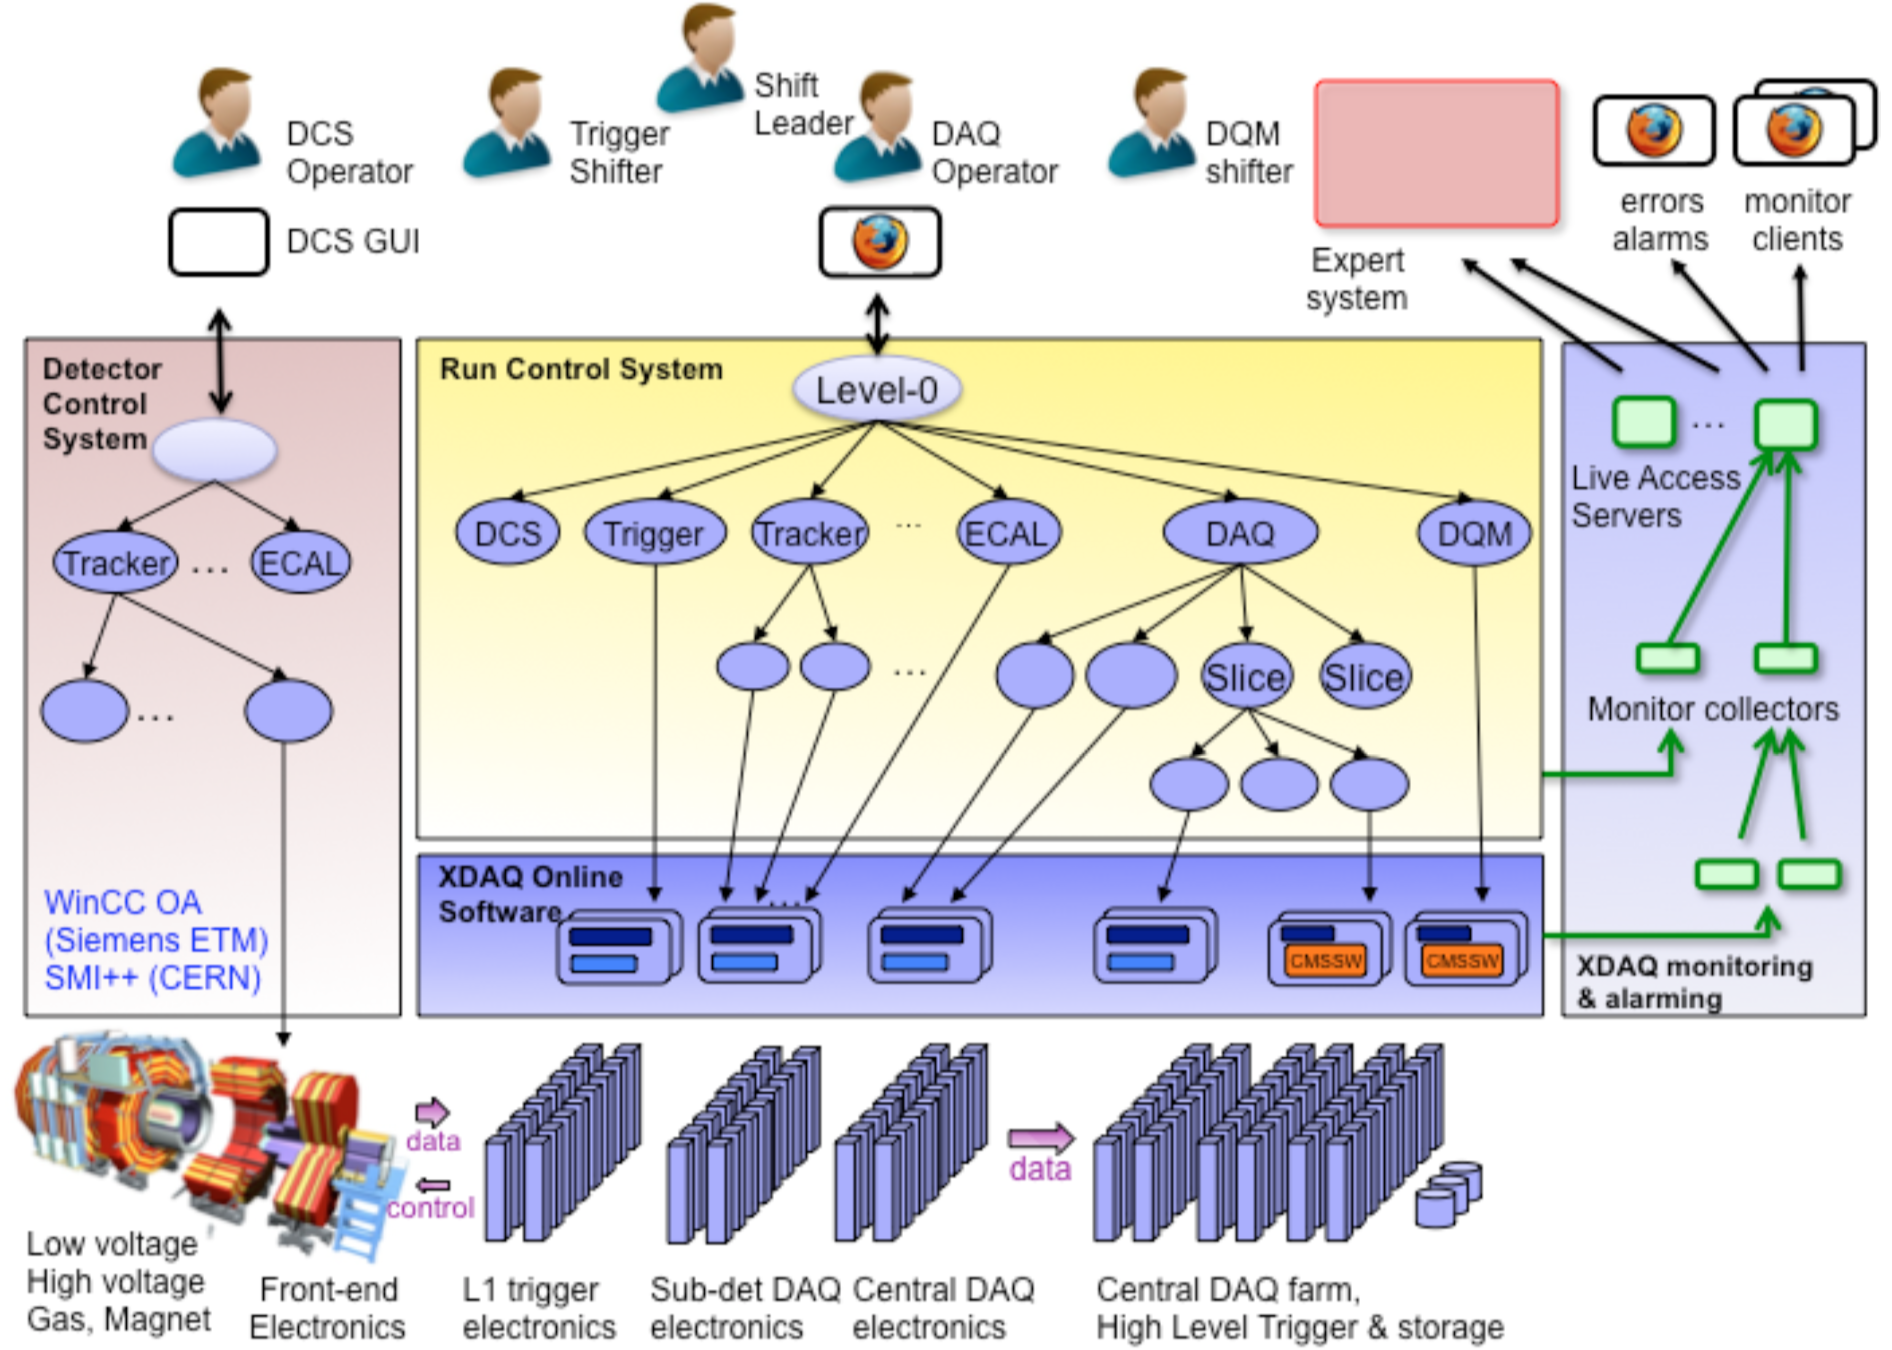
\includegraphics[width=\textwidth]{images/cms_online_system.png}
    \caption{Overview of the CMS online systems. Image retrieved from \cite{cms_daq}}
    \label{fig:cms_online_system}
\end{figure}

\subsection{Data Granularity}

We decide to divide a big chunk of data into one run and each run contain multiple lumisection which has an 23 seconds of interval due to the beam does not change much where we consider a 23 seconds of time.
Moreover, each lumisection contain multiple events. If we consider in term of time to reconstruction, there are Express and PromptReco where data are reconstructed at nearly real-time and two days after collision.

% \begin{table}[ht]
% \center
% \begin{tabular}{cc|c}
% A & B & A XOR B\\
% \hline
% 0 & 0 & 0\\
% 0 & 1 & 1\\
% 1 & 0 & 1\\
% 1 & 1 & 0\\
% \end{tabular}
% \caption{A simple table in \LaTeX.}
% \label{tab:xor}
% \end{table}


%%%%%%%%%%%%%%%%%%%%%%
%     CMS-DQM
%%%%%%%%%%%%%%%%%%%%%%

\section{Data Quality Monitoring (DQM)}

In order to make sure that data quality is nearly perfectly well collected, there is another story called DQM where it's actually the subset of the run control system in the Figure \ref{fig:cms_online_system}.
CMS DQM team provide the tool where there is online and offline shifter checking the result from beam collision real-time and 48 hours after collision orderly. Figure \ref{fig:dqm_flow} is the schematic of DQM workflow where including the tools and person who responsible for each module.
If some sub-system went weird such as peak of the histogram drastically increase with no physical sense or some part of the detector turnoff, they will report in the log of the system in running process and calling detector experts to inspect the problem.
In this work, we will only focus on the red box which is the offline world.

\begin{figure}[h!]
    \centering
    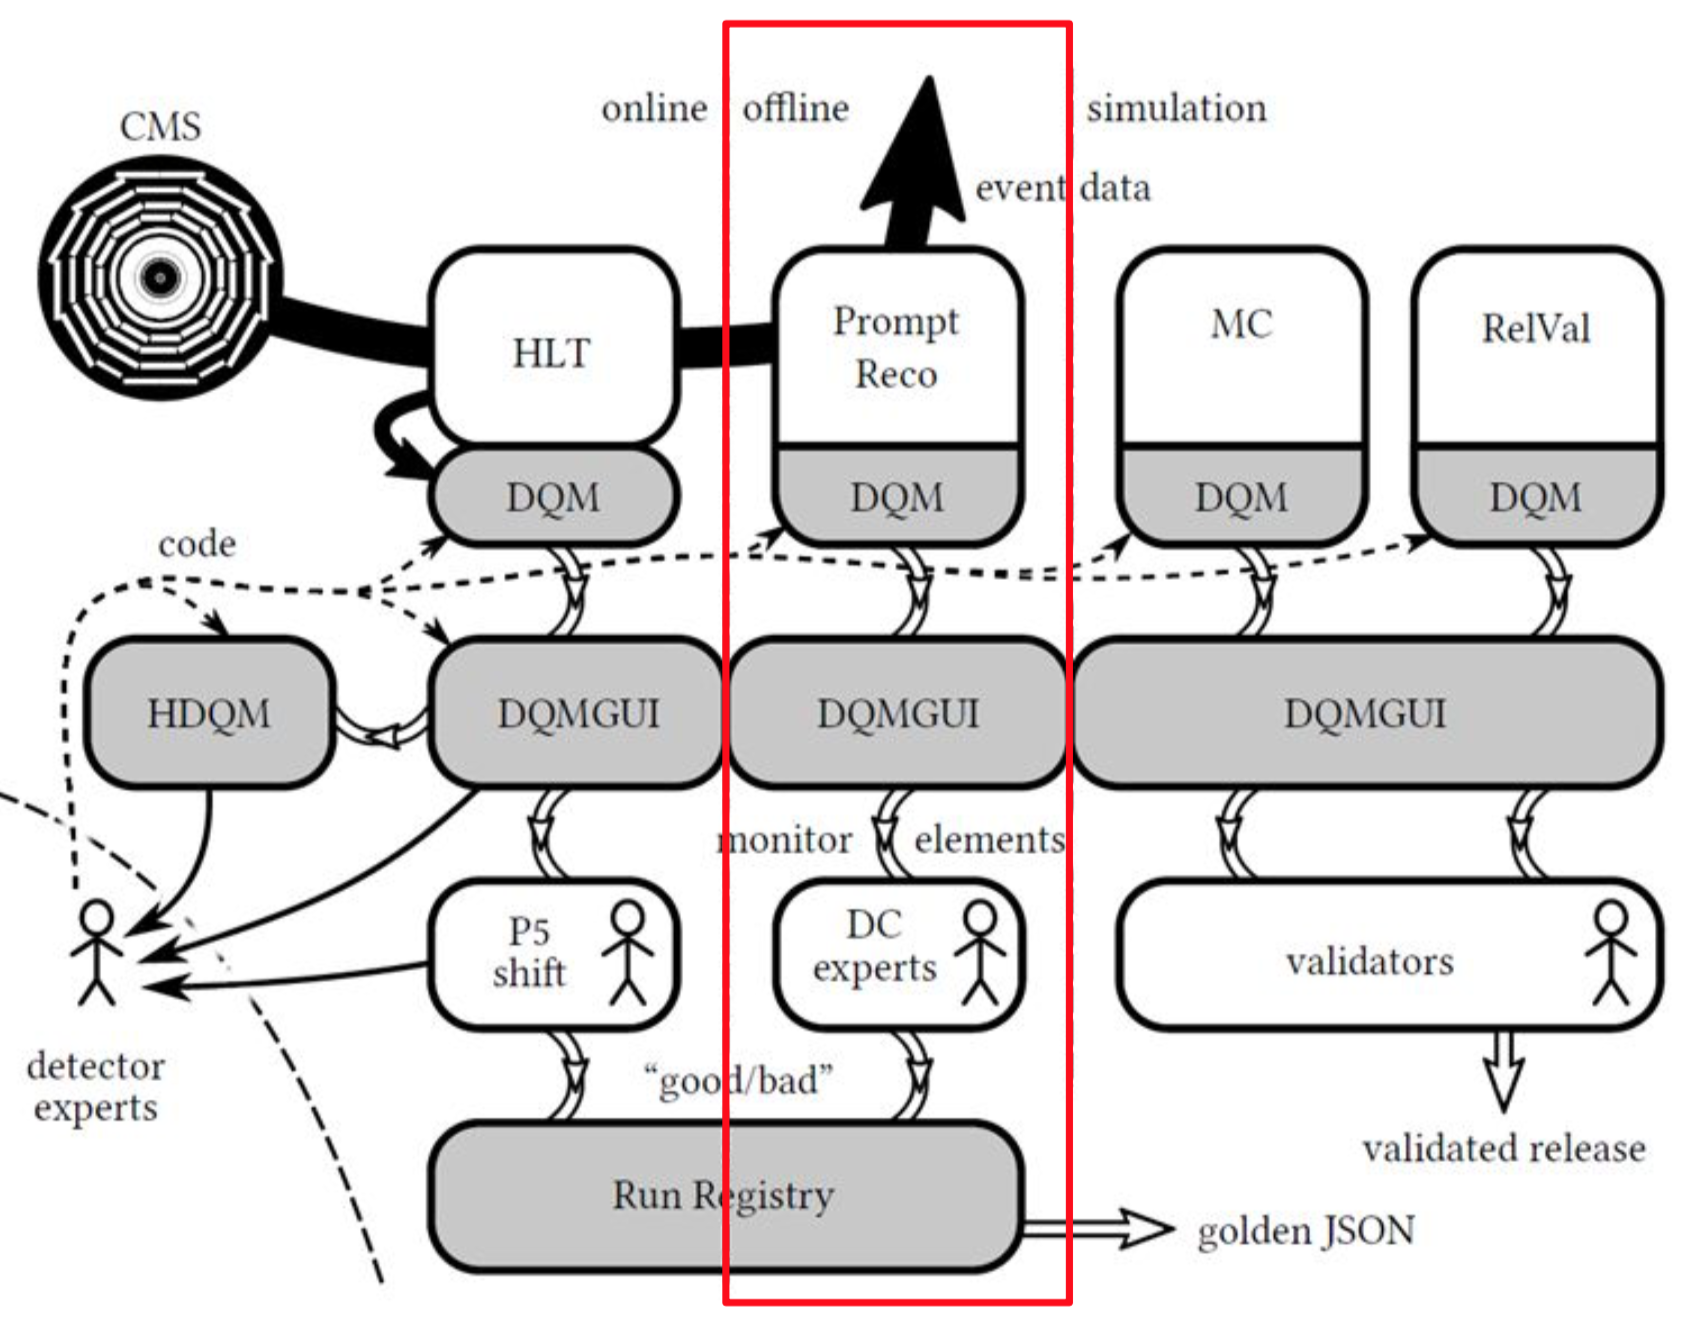
\includegraphics[width=0.7\textwidth]{images/dqm_flow.png}
    \caption{Tools and Processes of DQM. Image retrieved from M. Schneider, CHEP 2018}
    \label{fig:dqm_flow}
\end{figure}

Regarding the scope that we want to mimic, offline shifter and detector experts check a multiple distribution histogram to inspect and certify data quality.
The certification is made run and lumisection granularity. The procedure to certify the data are the following list
\begin{enumerate}
    \item Runs tagged as bad by human (whole run)
    \item Automatically filter by DCS bits, beam status and etc. (LS levels)
    \item In rare cases are marked by DC experts (LS levels)
\end{enumerate}
Then the rest of them that pass all of those criteria are defined in Golden JSON which are all of good LS.






\chapter{Objectives}

\lipsum % replace with your text

\section{Expectation}

\lipsum % replace with your text

\section{Proposal For an Alternative Approach}

\lipsum % replace with your text
\chapter{Methodology}

\lipsum  % Replace with your text


\section{Datasets}

\subsection{Histogram Representation}
\lipsum  % Replace with your text

\subsection{Data Preprocessing}
\lipsum  % Replace with your text

\section{Semi-Supervised Learning}

\lipsum  % Replace with your text


\subsection{Sch\"{o}lkopf's One-Class SVM}

\lipsum  % Replace with your text


\subsection{Isolation Forest}

\lipsum  % Replace with your text

\subsection{Autoencoder}

\lipsum  % Replace with your text

\subsubsection{Vanilla}
\subsubsection{Sparse}
\chapter{Results and Interpretation}

%%%%%%%%%%%%%%%%%
%     2016
%%%%%%%%%%%%%%%%%
\section{2016 Datasets}

\subsection{Primary Analysis}
In order to roughly understand a group (similar patterns) of data, one way to do it is to reduce the dimension of data. In our case, there are 259 features which will be transformed into two-dimension on the basis of two eigenvectors (selected by two largest eigenvalues) belonging to covariance matrix which computed from the datasets.
\begin{figure}[h!]
    \centering
    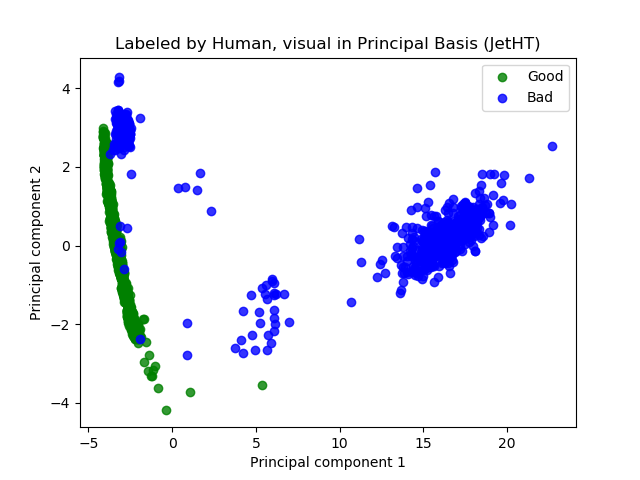
\includegraphics[width=0.6\textwidth]{images/reco/2016/JetHT_label_2016.png}
    \caption{Principal component with the labeled color from the system}
    \label{fig:JetHT_label_2016}
\end{figure}

As it can be seen on the green line in Figure \ref{fig:JetHT_label_2016} that there are nice band which is good LS and a few weird LSs that located outside the tubular shape as well as bad LS that could be divided into the bad LS with some patterns and anomaly bad LS which I would call both of them as "outlier". That's essentially the punchline why I called outlier detection instead of anomaly detection.

\subsection{Performance}
By Iteratively retrain the model ten times to make sure that it's working systematically and plot the root mean square as a shady fluctuation in Figure \ref{fig:performance_2016}
\begin{figure}[h!]
\centering
    \begin{subfigure}[b]{0.49\linewidth}
        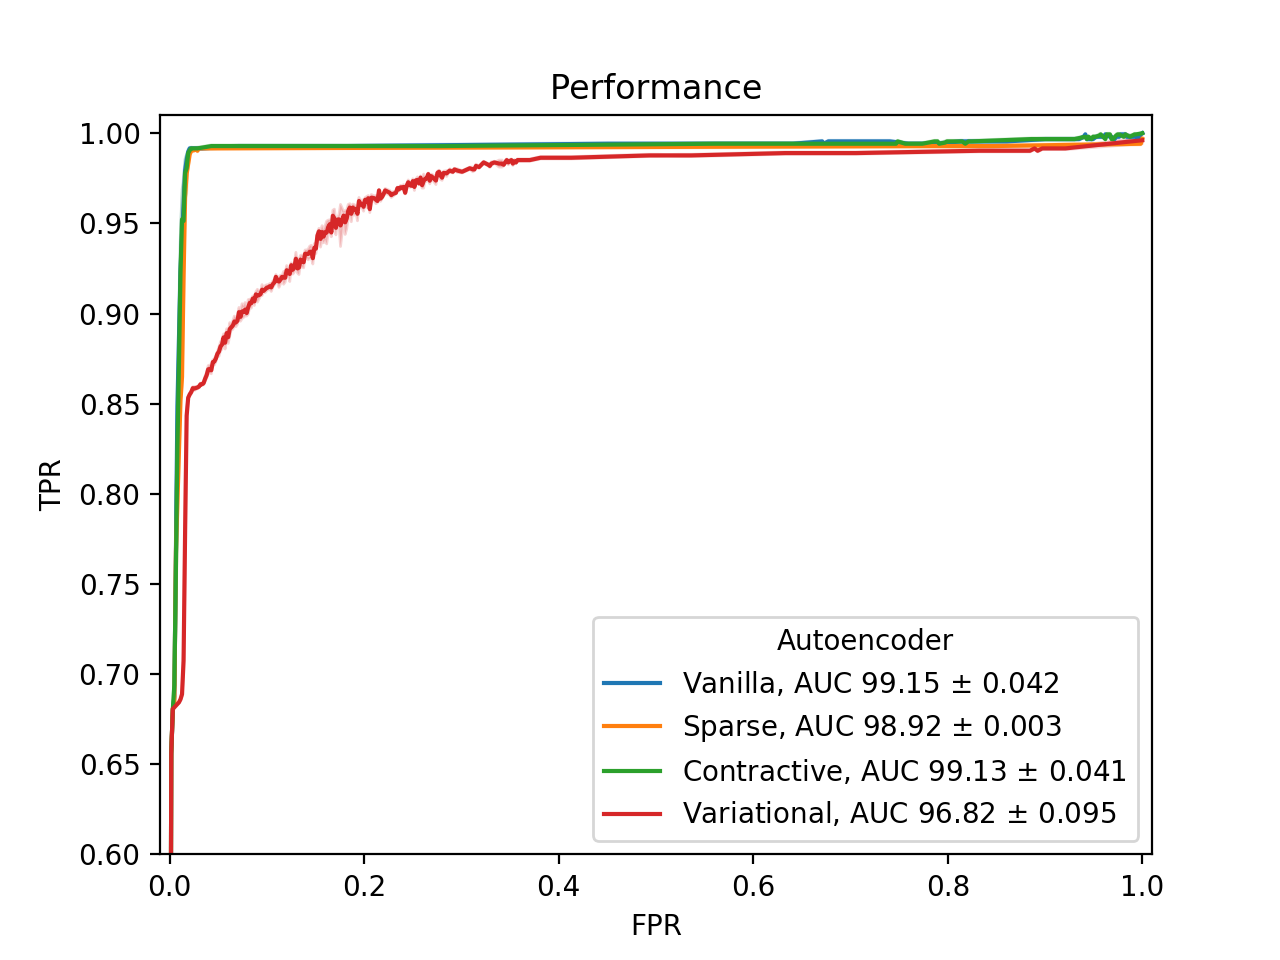
\includegraphics[width=\linewidth]{images/reco/2016/performance.png}
        \caption{4 Flavours of AE}
    \end{subfigure}
    \begin{subfigure}[b]{0.49\linewidth}
        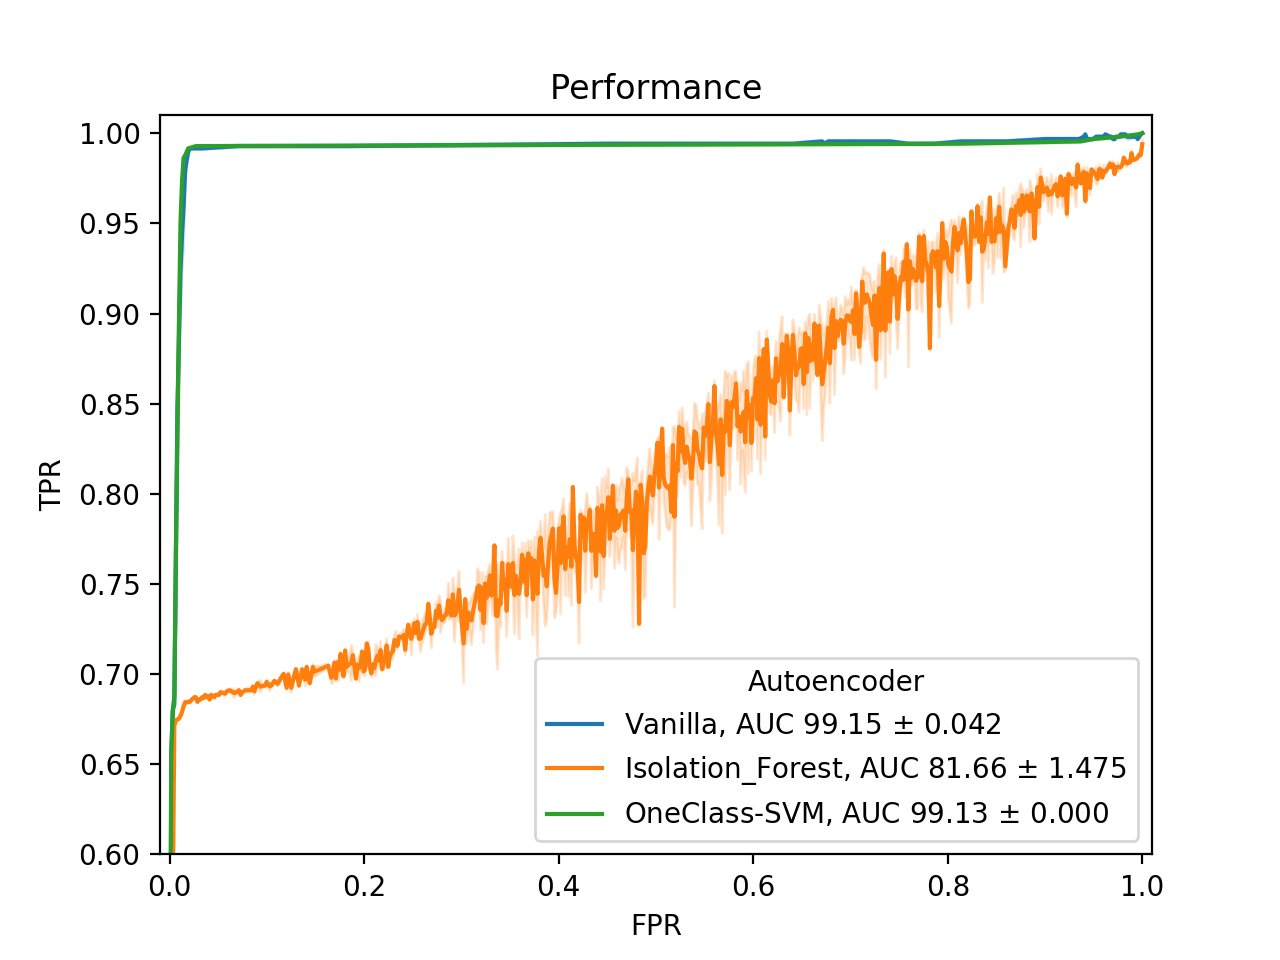
\includegraphics[width=\linewidth]{images/reco/2016/performance_ml.png}
        \caption{Vanilla AE vs SVM vs Isolation Forest}
    \end{subfigure}
\caption{Comparative visualization of model performance}
\label{fig:performance_2016}
\end{figure}

To sum up, even there are a fancy mathematical expression of non-vanilla autoencoders but it does not guarantee that we would get the best performance out of it. On the other hand, the simplest AE has the performance among all AE. One other interesting spot is the performance of OneClass-SVM also yields the remarkable results as nearly compatible with Vanilla AE without any fluctuation since the model itself has no randomness and work very straightforward.

\subsection{Distribution of decision value (to find the threshold)}
The story behind the performance figure is genuinely extracted from the distribution of decision value from Figure \ref{fig:2016_decision_value_dist} and slowly moving a threshold of minimal point in the overlapping region of good and bad LS from a label in the distribution until it got the maximal value. The below figures are the comparison between our two great candidates by considering to pick some threshold and see the contamination on each side.

\begin{figure}[h!]
    \centering
    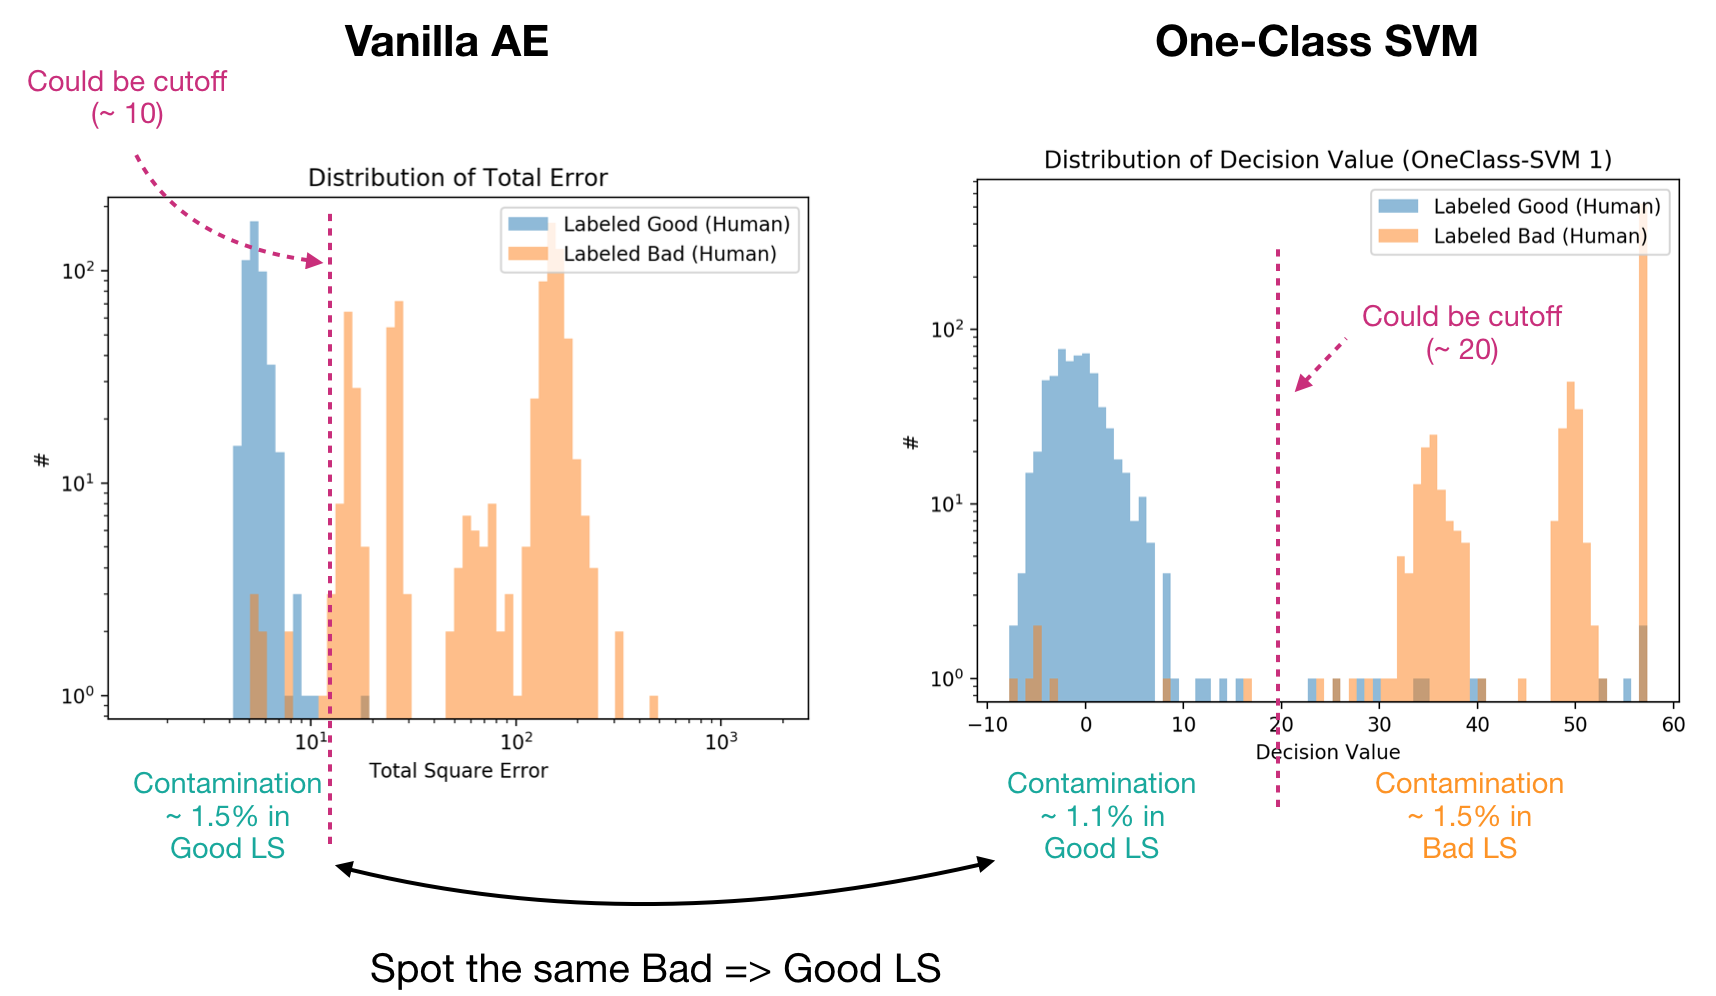
\includegraphics[width=\textwidth]{images/reco/2016/decision_value_dist.png}
    \caption{Distribution of decision value}
    \label{fig:2016_decision_value_dist}
\end{figure}

For Vanilla AE, the contamination of bad LS falling into good LS is around 1\% over the good LS below the cutoff and there are only a few of good LS falling into bad LS which might be ignorable.

For OneClass-SVM, the contamination LS that bad falling into good LS is almost the same as Vanilla AE does. There is no coincidence for a totally different approach of model train and spot the same thing. This might implicitly imply that it either came from some imperfection of data in the training and testing or some kind of malfunction in the sub-system could not propagate into JetHT physics objects.

As can be seen in the distribution, there is no clear grey zone for this study so far.

\subsection{Example of square error from reconstruction}
Figure \ref{fig:2016_example_se} shows the example of LS reconstruction which calculated from $x$ and $\tilde{x}$ between good and bad LS.
\begin{figure}[h!]
    \centering
    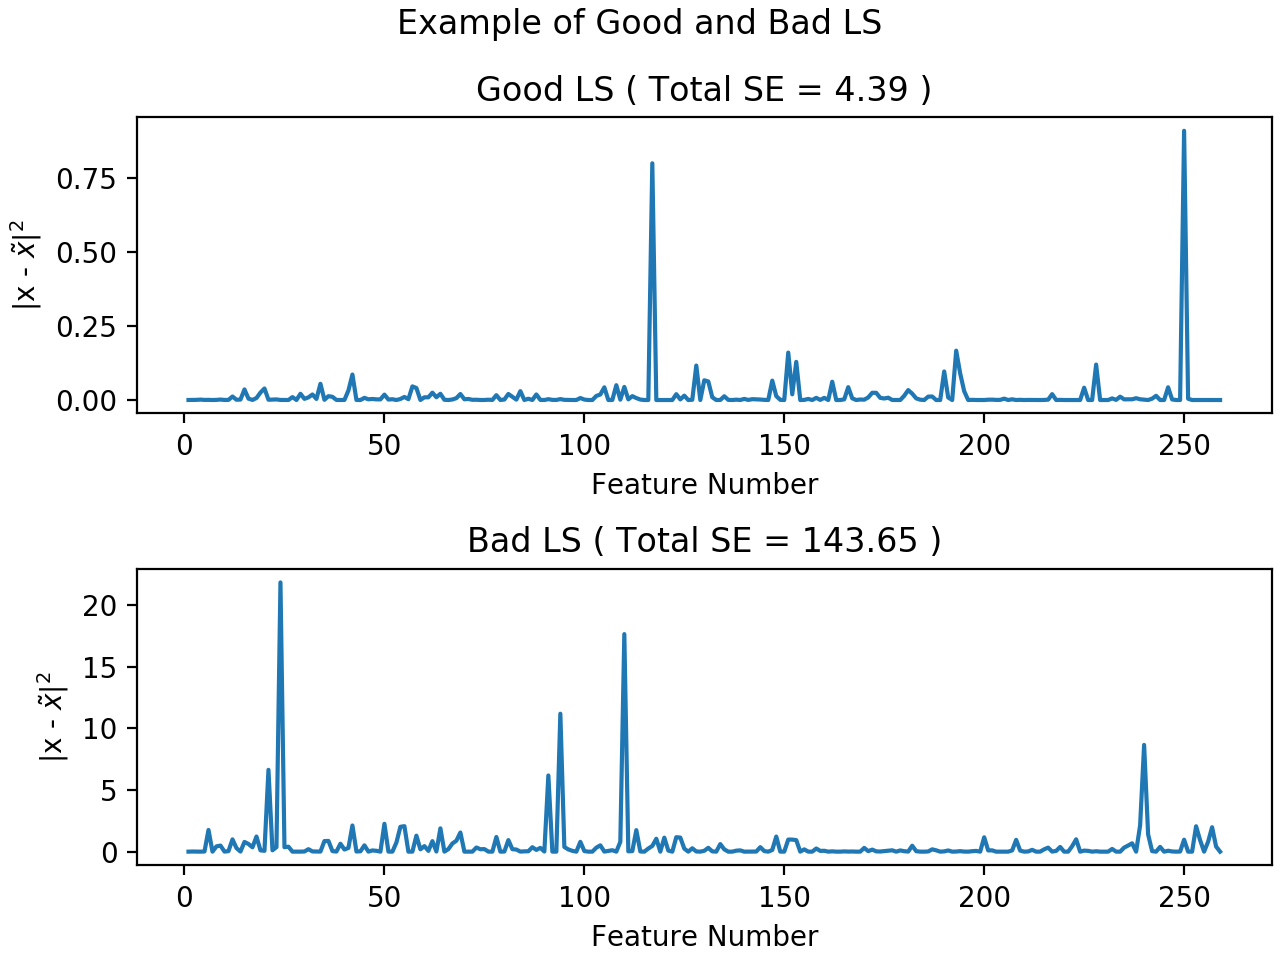
\includegraphics[width=0.8\textwidth]{images/reco/2016/example_se.png}
    \caption{Reconstruction error from Vanilla AE}
    \label{fig:2016_example_se}
\end{figure}

\subsection{Extended Investigation}
It may be questioned why many of bad LS seems to have a group of bad LS as you have seen in the plot of hyperspace and few collections of bad LS in decision value distribution (As the black arrow that links between the distribution and 2D-hyperspace). In this section, I want to explicitly prove that the model really sees that the right cluster is the worse bad LS and closer to tubular is less bad LS which decision value has to be quite similar to good LS. In order to prove that, I choose our best candidate to shade the decision value as z-axis color to represent how bad LS in each data point is as in Figure \ref{fig:2016_guess_visual}. The result strongly agrees that there are obvious bad lumisection and less badness as it gets closer to the green band.
\begin{figure}[h!]
    \centering
    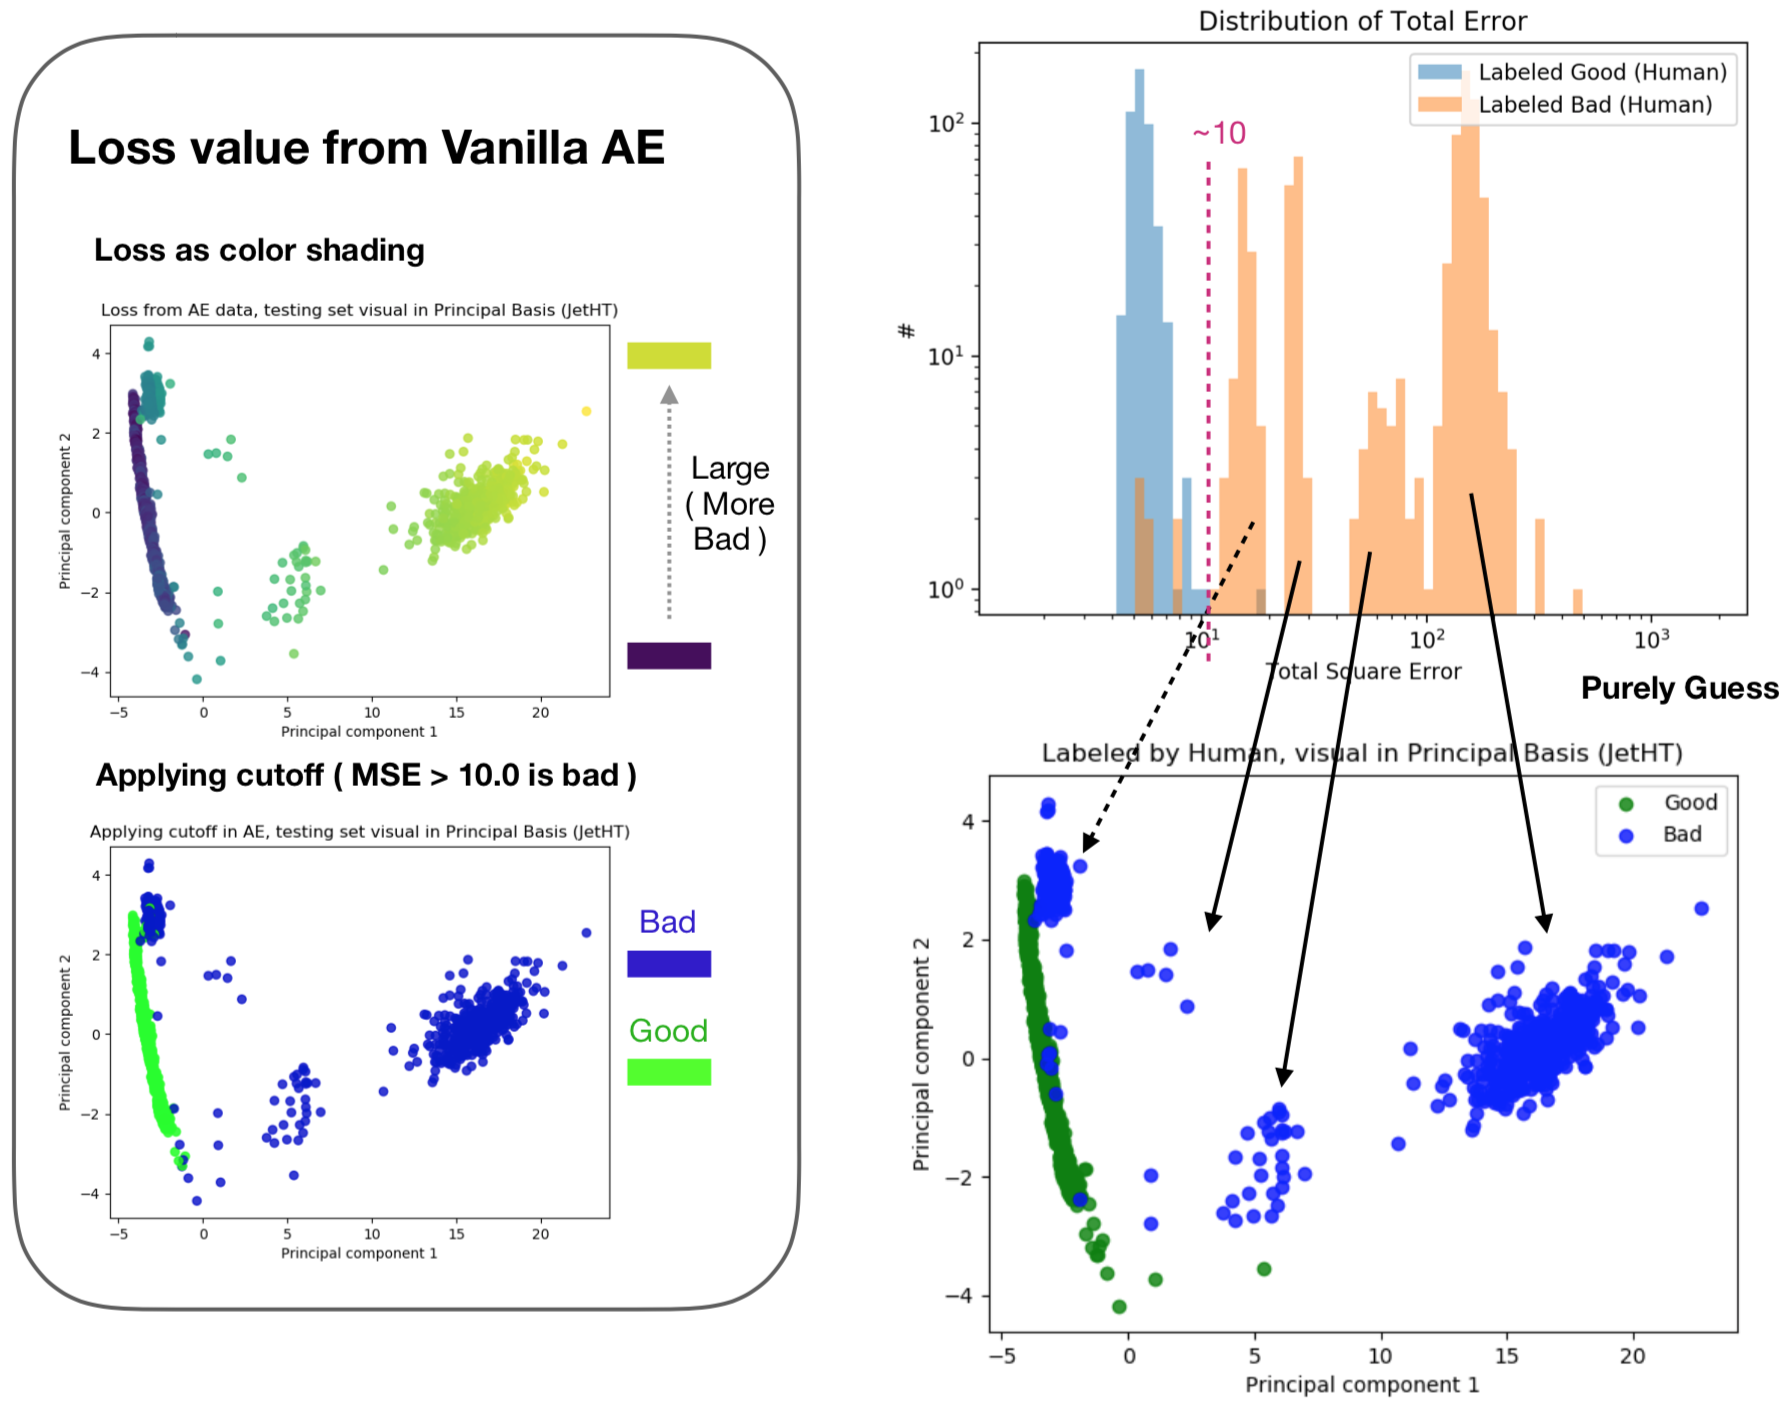
\includegraphics[width=\textwidth]{images/reco/2016/guess_visual.png}
    \caption{Colorize reconstruction error from Vanilla AE}
    \label{fig:2016_guess_visual}
\end{figure}


%%%%%%%%%%%%%%%%%
%     2018
%%%%%%%%%%%%%%%%%

\section{2018 Datasets}

\subsection{Primary Analysis}
For 2018 data, we dig a bit more to understand which cause the badness of bad LS by taking sub-system label into account from RR's API. There is plenty of sub-systems in CMS detector. In order to roughly understand the malfunction of sub-system, we decided to pull label only for HCAL, ECAL, TRACKER and MUON detector which are the main part of the detector.

To roughly describe each feature contribute to each principal component, we extract the element in matrix transform (equivalent to an element in each eigenvector) and take the absolute value to consider only for the magnitude and ignore the direction in the space where it directly proportional to the contribution of each one.
The spectrum of contribution will provide in the following hyperspace of each primary dataset.

\begin{figure}[h!]
\centering
    \begin{subfigure}[b]{0.49\linewidth}
        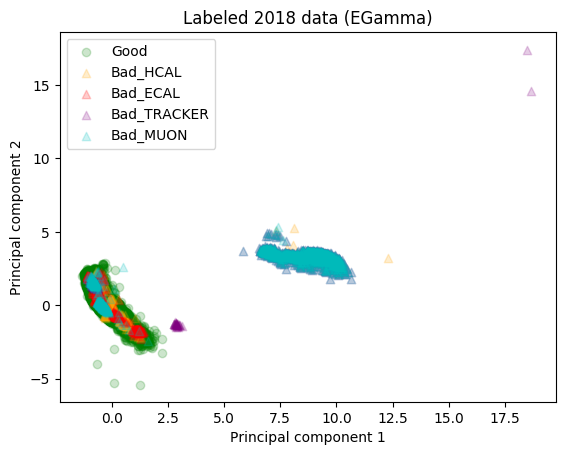
\includegraphics[width=\linewidth]{images/reco/2018/EGamma_subsystem_label.png}
        \caption{Full range}
    \end{subfigure}
    \begin{subfigure}[b]{0.49\linewidth}
        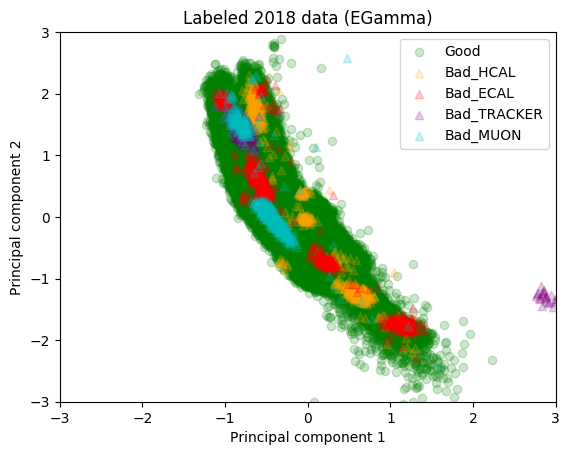
\includegraphics[width=\linewidth]{images/reco/2018/EGamma_subsystem_label_short_range.png}
        \caption{Zoom in}
    \end{subfigure}
    \begin{subfigure}[b]{0.49\linewidth}
        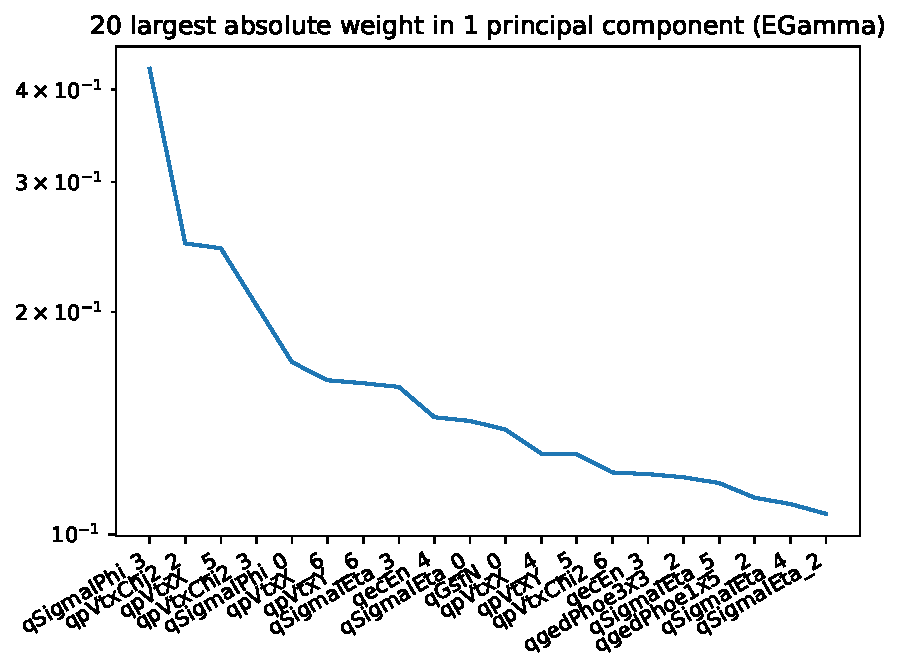
\includegraphics[width=\linewidth]{images/reco/2018/feature_2/EGamma_pc1.pdf}
        \caption{Contribution of features on PC1 \\ (explained variance ratio = 0.31)}
    \end{subfigure}
    \begin{subfigure}[b]{0.49\linewidth}
        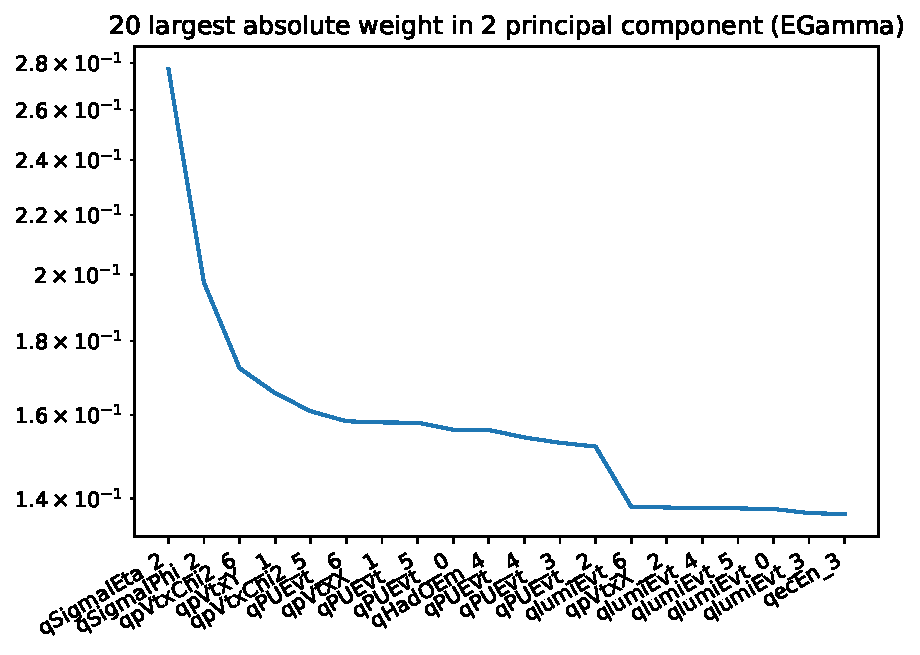
\includegraphics[width=\linewidth]{images/reco/2018/feature_2/EGamma_pc2.pdf}
        \caption{Contribution of features on PC2 \\ (explained variance ratio = 0.25)}
    \end{subfigure}
\caption{Two principal components of EGamma}
\label{fig:2018_EGamma_subsystem_label}
\end{figure}

\begin{figure}[h!]
\centering
    \begin{subfigure}[b]{0.49\linewidth}
        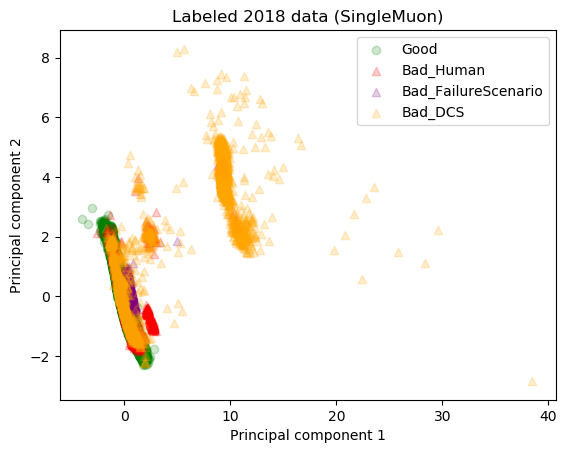
\includegraphics[width=\linewidth]{images/reco/2018/SingleMuon_label_separate.png}
        \caption{Full range}
    \end{subfigure}
    \begin{subfigure}[b]{0.49\linewidth}
        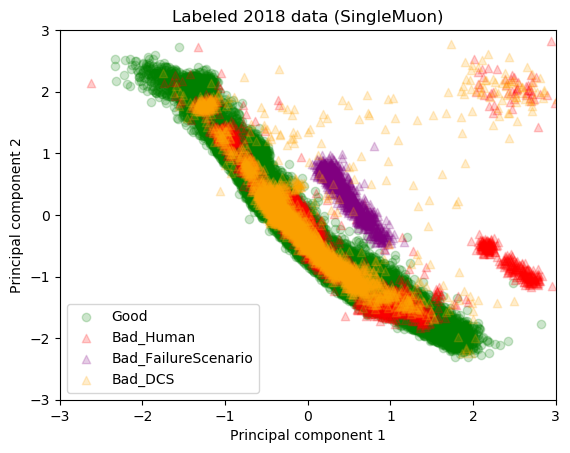
\includegraphics[width=\linewidth]{images/reco/2018/SingleMuon_label_separate_short_range.png}
        \caption{Zoom in}
    \end{subfigure}
    \begin{subfigure}[b]{0.49\linewidth}
        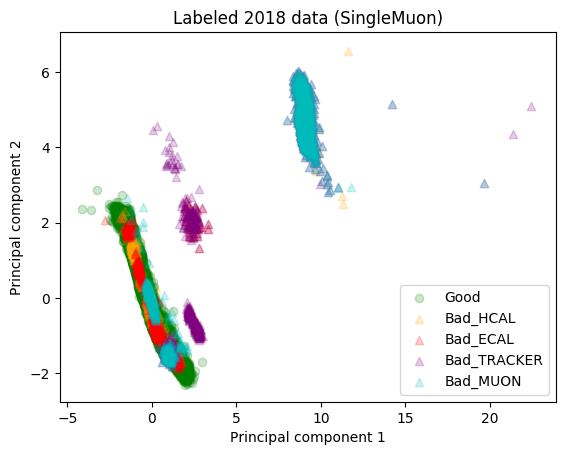
\includegraphics[width=\linewidth]{images/reco/2018/SingleMuon_subsystem_label.png}
        \caption{Full range}
    \end{subfigure}
    \begin{subfigure}[b]{0.49\linewidth}
        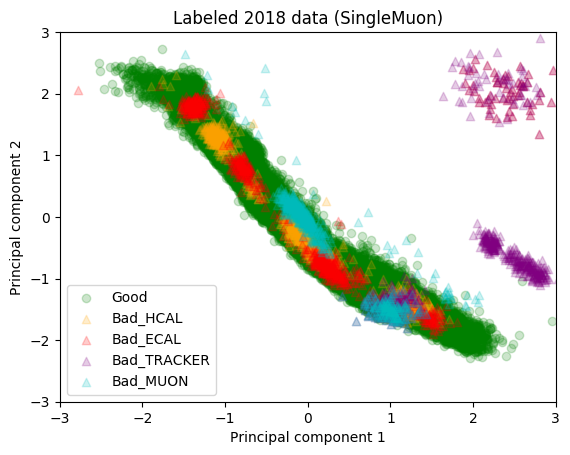
\includegraphics[width=\linewidth]{images/reco/2018/SingleMuon_subsystem_label_short_range.png}
        \caption{Zoom in}
    \end{subfigure}
    \begin{subfigure}[b]{0.49\linewidth}
        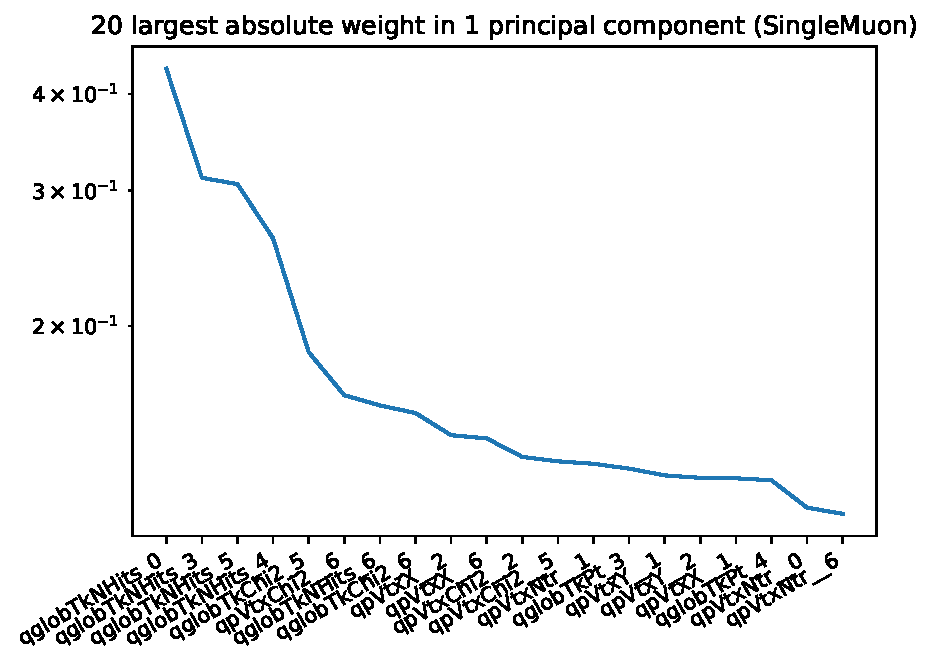
\includegraphics[width=\linewidth]{images/reco/2018/feature_2/SingleMuon_pc1.pdf}
        \caption{Contribution of features on PC1 \\ (explained variance ratio = 0.37)}
    \end{subfigure}
    \begin{subfigure}[b]{0.49\linewidth}
        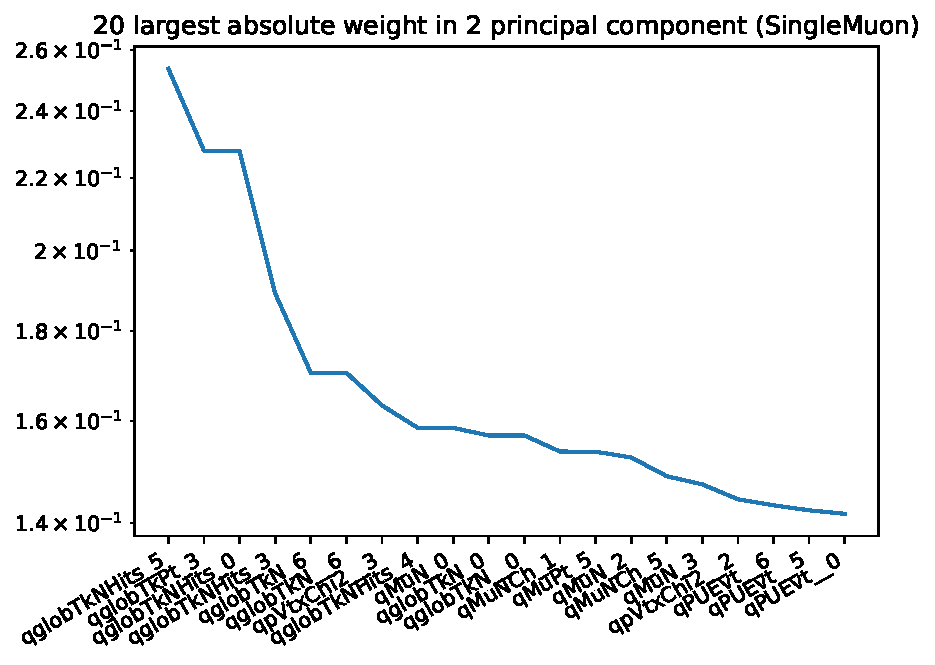
\includegraphics[width=\linewidth]{images/reco/2018/feature_2/SingleMuon_pc2.pdf}
        \caption{Contribution of features on PC2 \\ (explained variance ratio = 0.22)}
    \end{subfigure}
    \caption{Two principal components of Single Muon}
\label{fig:2018_SingleMuon_subsystem_label}
\end{figure}


\begin{figure}[h!]
\centering
    \begin{subfigure}[b]{0.49\linewidth}
        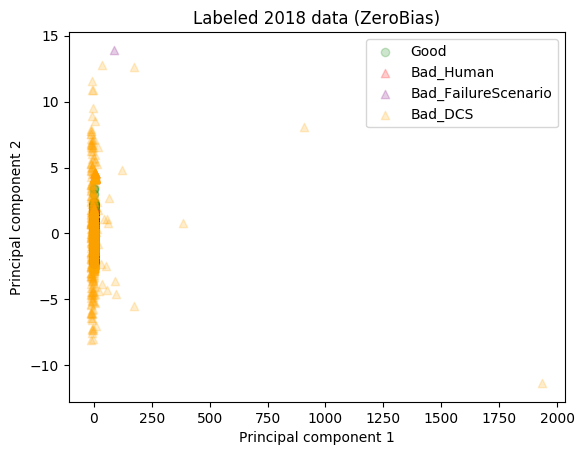
\includegraphics[width=\linewidth]{images/reco/2018/ZeroBias_label_separate.png}
        \caption{Full range}
    \end{subfigure}
    \begin{subfigure}[b]{0.49\linewidth}
        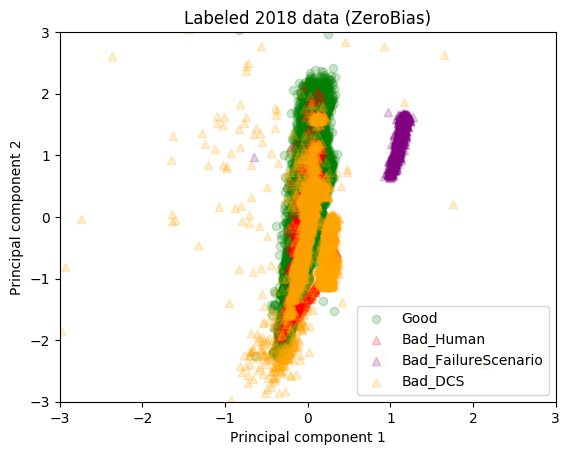
\includegraphics[width=\linewidth]{images/reco/2018/ZeroBias_label_separate_short_range.png}
        \caption{Zoom in}
    \end{subfigure}
    \begin{subfigure}[b]{0.49\linewidth}
        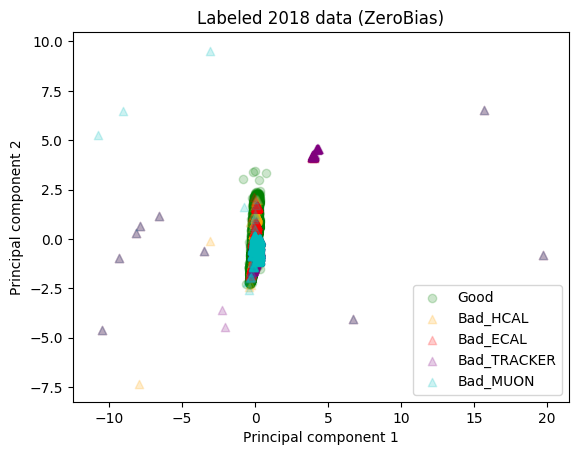
\includegraphics[width=\linewidth]{images/reco/2018/ZeroBias_subsystem_label.png}
        \caption{Full range}
    \end{subfigure}
    \begin{subfigure}[b]{0.49\linewidth}
        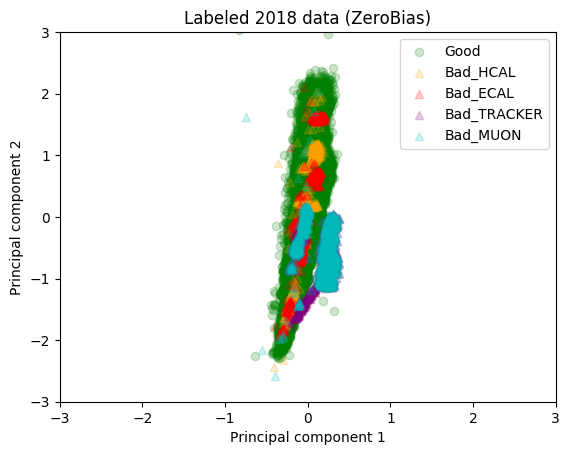
\includegraphics[width=\linewidth]{images/reco/2018/ZeroBias_subsystem_label_short_range.png}
        \caption{Zoom in}
    \end{subfigure}
    \begin{subfigure}[b]{0.49\linewidth}
        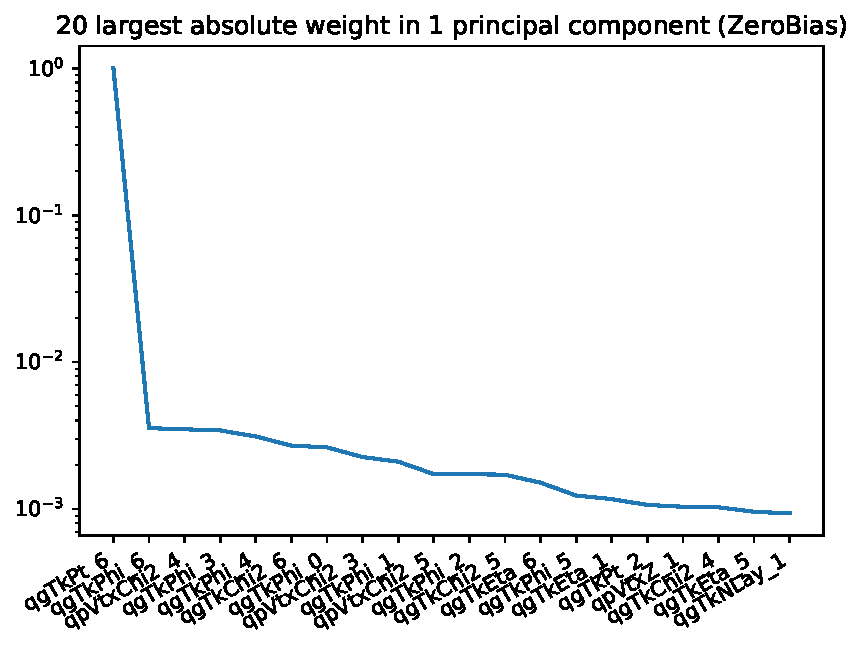
\includegraphics[width=\linewidth]{images/reco/2018/feature_2/ZeroBias_pc1.pdf}
        \caption{Contribution of features on PC1 \\ (explained variance ratio = 0.89)}
    \end{subfigure}
    \begin{subfigure}[b]{0.49\linewidth}
        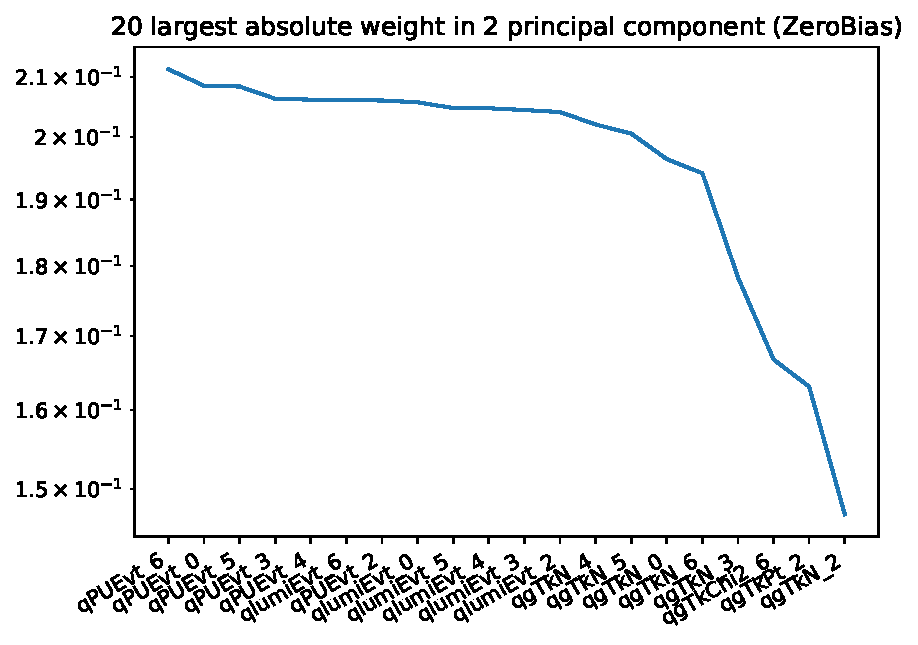
\includegraphics[width=\linewidth]{images/reco/2018/feature_2/ZeroBias_pc2.pdf}
        \caption{Contribution of features on PC2 \\ (explained variance ratio = 0.0225)}
    \end{subfigure}
    \caption{Two principal components of ZeroBias}
\label{fig:2018_ZeroBias_subsystem_label}
\end{figure}

\begin{figure}[h!]
\centering
    \begin{subfigure}[b]{0.49\linewidth}
        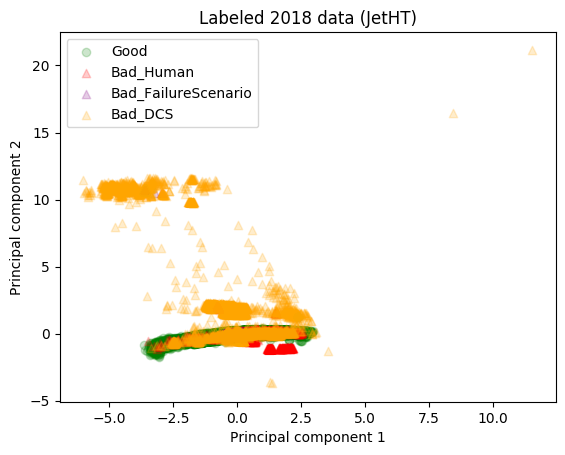
\includegraphics[width=\linewidth]{images/reco/2018/JetHT_label_separate.png}
        \caption{Full range}
    \end{subfigure}
    \begin{subfigure}[b]{0.49\linewidth}
        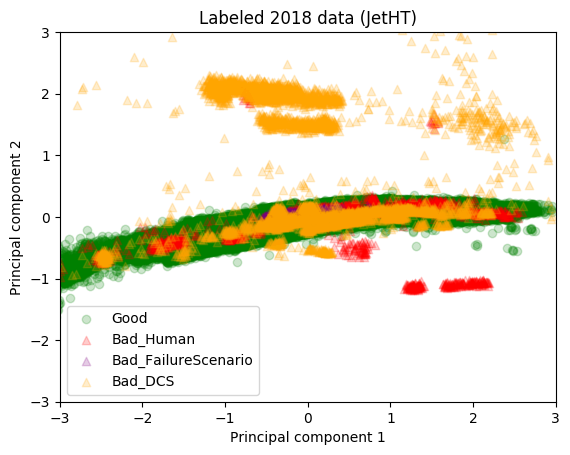
\includegraphics[width=\linewidth]{images/reco/2018/JetHT_label_separate_short_range.png}
        \caption{Zoom in}
    \end{subfigure}
    \begin{subfigure}[b]{0.49\linewidth}
        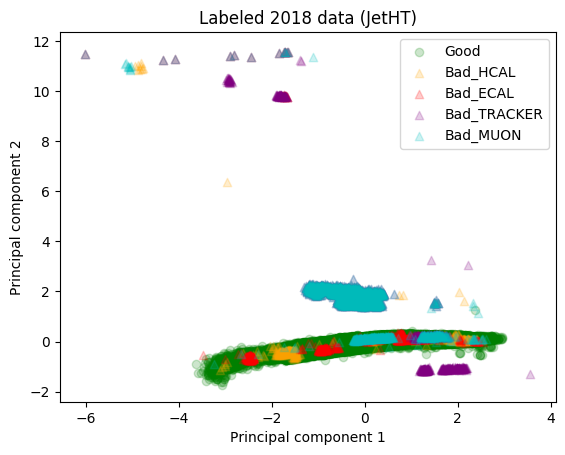
\includegraphics[width=\linewidth]{images/reco/2018/JetHT_subsystem_label.png}
        \caption{Full range}
    \end{subfigure}
    \begin{subfigure}[b]{0.49\linewidth}
        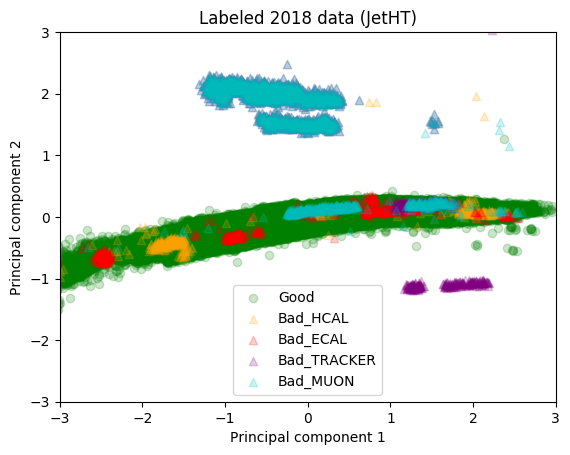
\includegraphics[width=\linewidth]{images/reco/2018/JetHT_subsystem_label_short_range.png}
        \caption{Zoom in}
    \end{subfigure}
    \begin{subfigure}[b]{0.49\linewidth}
        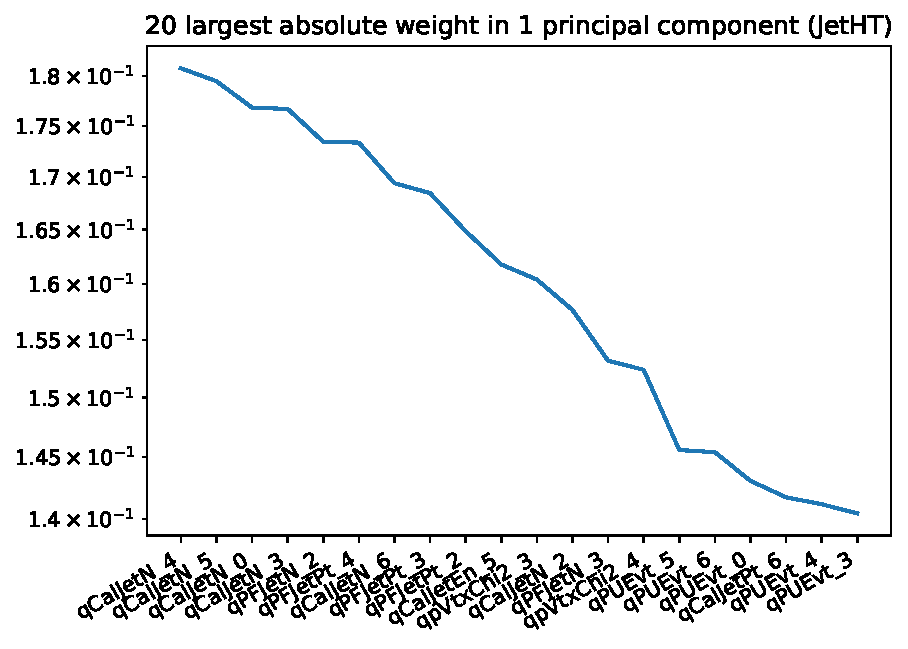
\includegraphics[width=\linewidth]{images/reco/2018/feature_2/JetHT_pc1.pdf}
        \caption{Contribution of features on PC1 \\ (explained variance ratio = 0.45)}
    \end{subfigure}
    \begin{subfigure}[b]{0.49\linewidth}
        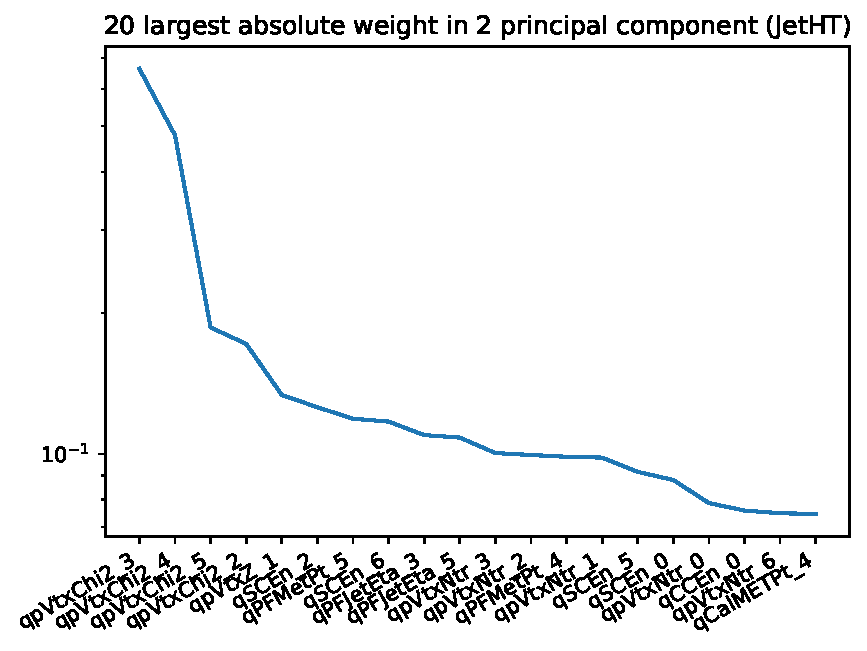
\includegraphics[width=\linewidth]{images/reco/2018/feature_2/JetHT_pc2.pdf}
        \caption{Contribution of features on PC2 \\ (explained variance ratio = 0.21)}
    \end{subfigure}
    \caption{Two principal components of JetHT}
\label{fig:2018_JetHT_subsystem_label}
\end{figure}

According to Figure (\ref{fig:2018_EGamma_subsystem_label}, \ref{fig:2018_SingleMuon_subsystem_label}, \ref{fig:2018_ZeroBias_subsystem_label}, \ref{fig:2018_JetHT_subsystem_label}), It's obviously to tell that the cluster of outlier are mainly consists of malfunction from MUON and TRACKER sub-detector. Not only the outlier that has an interesting pattern but clustering in inlier is also remarkably considerable as clustering mainly from a malfunction of ECAL and HCAL that located near or inside the green band.

Please note that the calculation of the matrix transform exclude failure scenario since it's a fake data and it might leading to a weird correlation in covariance matrix.
The following list is the list of important features that highly correlated to the rest of them in our dataset
\begin{itemize}
    \item From Figure \ref{fig:2018_EGamma_subsystem_label}, qpVt in transverse direction and qSigmalEta contribute in first component.
    Secondly, second component mostly consists of qPUEvt and qlumiEvt. Lastly, there are overlapping feature where both of them sharing the different value which are qSigmalPhi and qpVtxChi2.
    \item Regarding Figure \ref{fig:2018_SingleMuon_subsystem_label}, qglobTkChi2 and qpVtx in perpendicular direction of the beam are dominated in first component and second component mostly consists of qPUEvt, qMuN and qMuNCh orderly.
    The only overlapping feature in SingleMuon is qglobTkNHits.
    \item For ZeroBias in Figure \ref{fig:2018_ZeroBias_subsystem_label}, both qgTkPt and qgTkPhi highly dominate in first component.
    Second component has smaller correlation which the faetures are qPUEvt, qlumiEvt and qgTkN.
    \item First component are constantly diminated to qCalJetN, qCalJetPt and qPUEvt orderly according to Figure \ref{fig:2018_JetHT_subsystem_label}.
    Feature qpVtxChi2, qPFMetPt and qPFJetEta also fairly equally contribute to the second component. 
\end{itemize}

\subsection{Performance}
\subsubsection{1) Include low statistics (fill null with zero) and testing with only bad LS form human}
Train with feature set 1 and the result has shown in Figure \ref{fig:2018_f1_ae_performance}.

The performance of AE for EGamma primary dataset is totally inefficient and even worse than randomly picking up which means that the model even saw most of bad LS even looks better than many good LS in the testing datasets. The rest of them is fairly acceptable but still not enough to exploit in the real system. Another interesting spot is the performance between a couple of AE in SingleMuon PD. 

\begin{figure}[h!]
\centering
    \begin{subfigure}[b]{0.49\linewidth}
        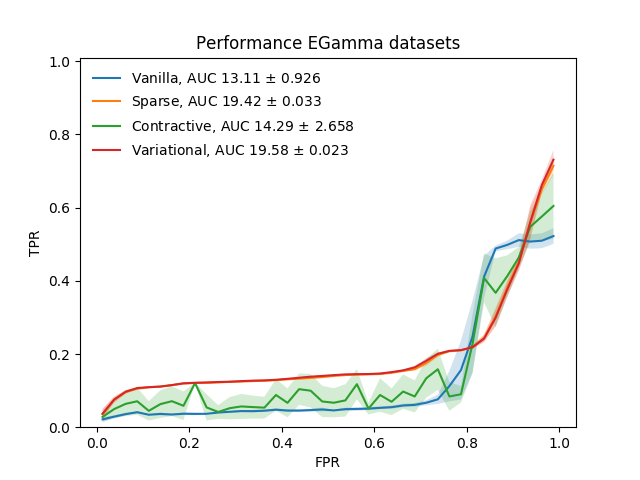
\includegraphics[width=\linewidth]{images/reco/2018/feature_1/performance_EGamma_VanillaSparseContractiveVariational.png}
        \caption{EGamma}
    \end{subfigure}
    \begin{subfigure}[b]{0.49\linewidth}
        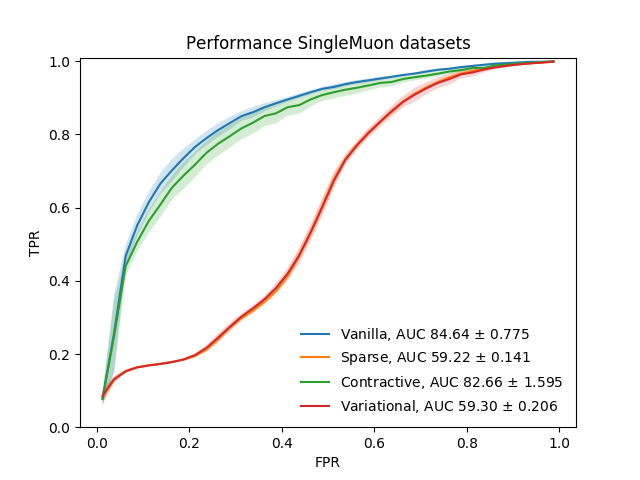
\includegraphics[width=\linewidth]{images/reco/2018/feature_1/performance_SingleMuon_VanillaSparseContractiveVariational.png}
        \caption{SingleMuon}
    \end{subfigure}
    \begin{subfigure}[b]{0.49\linewidth}
        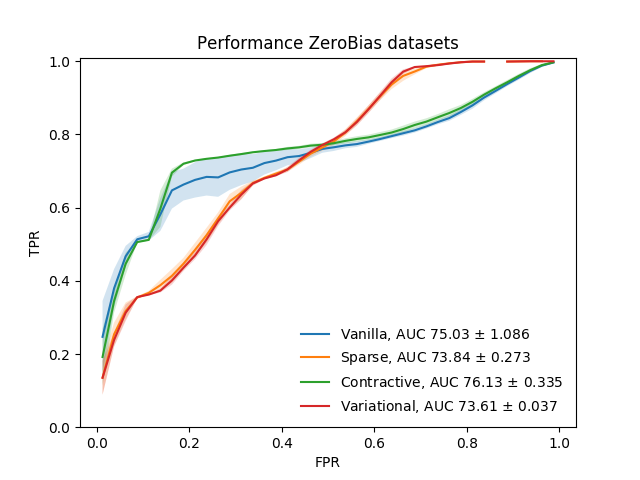
\includegraphics[width=\linewidth]{images/reco/2018/feature_1/performance_ZeroBias_VanillaSparseContractiveVariational.png}
        \caption{ZeroBias}
    \end{subfigure}
    \begin{subfigure}[b]{0.49\linewidth}
        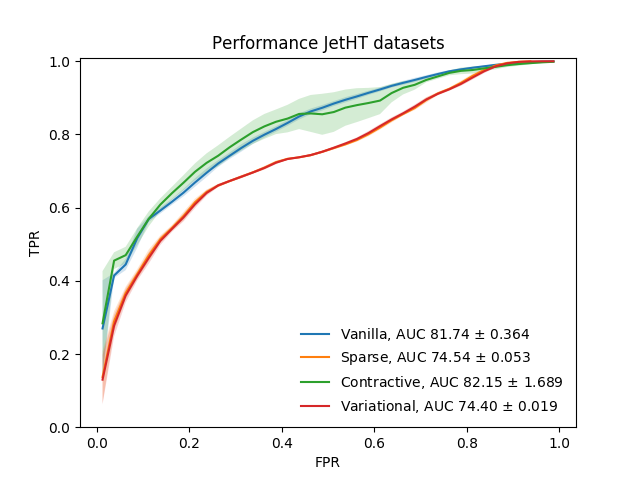
\includegraphics[width=\linewidth]{images/reco/2018/feature_1/performance_JetHT_VanillaSparseContractiveVariational.png}
        \caption{JetHT}
    \end{subfigure}
    \caption{Model performance for feature set 1 with 2018 data}
\label{fig:2018_f1_ae_performance}
\end{figure}

Figure \ref{fig:2018_f1_exteded_ae_performance} has demonstrated that even extended model has been combined various constraints that we know but it still not improves any further in terms of performance. Nevertheless, it has remarkable stability, especially for ContractiveVariational AE.

\begin{figure}[h!]
\centering
    \begin{subfigure}[b]{0.49\linewidth}
        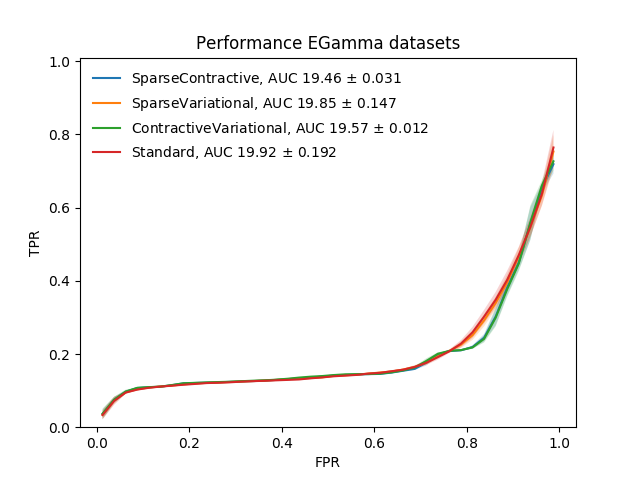
\includegraphics[width=\linewidth]{images/reco/2018/feature_1/performance_EGamma_SparseContractiveSparseVariationalContractiveVariationalStandard.png}
        \caption{EGamma}
    \end{subfigure}
    \begin{subfigure}[b]{0.49\linewidth}
        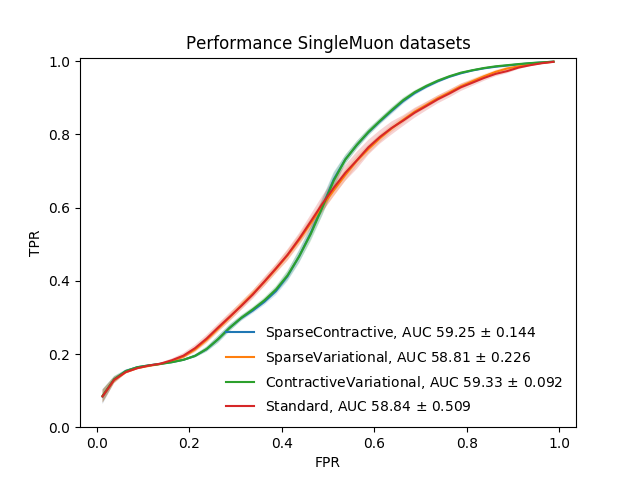
\includegraphics[width=\linewidth]{images/reco/2018/feature_1/performance_SingleMuon_SparseContractiveSparseVariationalContractiveVariationalStandard.png}
        \caption{SingleMuon}
    \end{subfigure}
    \begin{subfigure}[b]{0.49\linewidth}
        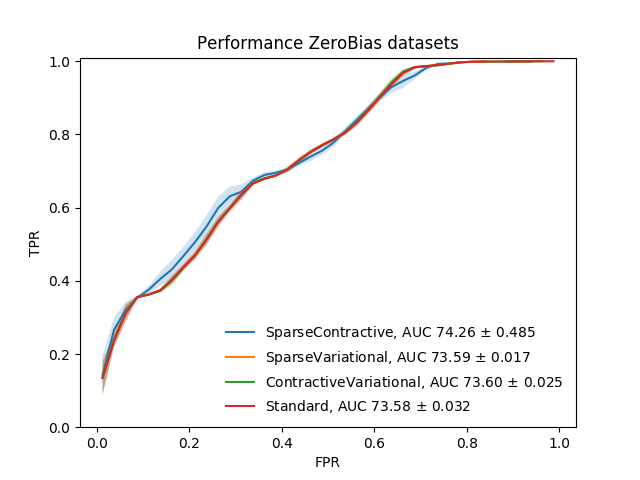
\includegraphics[width=\linewidth]{images/reco/2018/feature_1/performance_ZeroBias_SparseContractiveSparseVariationalContractiveVariationalStandard.png}
        \caption{ZeroBias}
    \end{subfigure}
    \begin{subfigure}[b]{0.49\linewidth}
        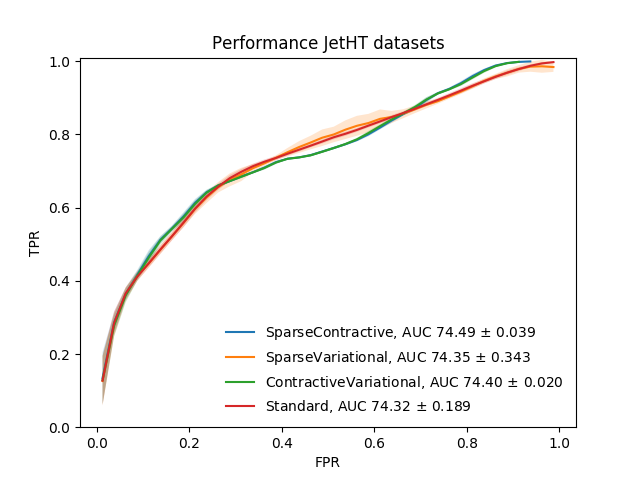
\includegraphics[width=\linewidth]{images/reco/2018/feature_1/performance_JetHT_SparseContractiveSparseVariationalContractiveVariationalStandard.png}
        \caption{JetHT}
    \end{subfigure}
    \caption{Extended model performance for feature set 1 with 2018 data}
\label{fig:2018_f1_exteded_ae_performance}
\end{figure}


\subsubsection{2) Exclude low statistics (Filter LS that has low EventsPerLs with value in the settings)}
Train with feature set 1 and the result has shown in Figure \ref{fig:2018_f2_ae_performance}.
We also perform an extended autoencoder for testing with this case, Figure \ref{fig:2018_f2_extended_ae_performance} has shown the stability and smoothness of the threshold as we have seen in Figure \ref{fig:2018_f1_exteded_ae_performance}.

\begin{figure}[h!]
\centering
    \begin{subfigure}[b]{0.49\linewidth}
        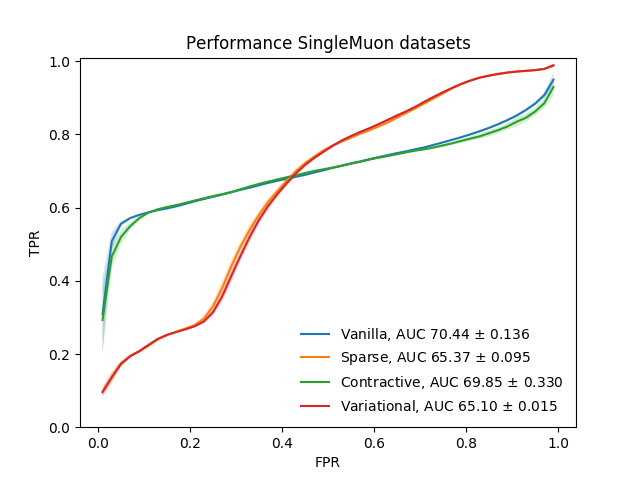
\includegraphics[width=\linewidth]{images/reco/2018/feature_2/performance_SingleMuon_VanillaSparseContractiveVariational.png}
        \caption{Full range}
    \end{subfigure}
    \begin{subfigure}[b]{0.49\linewidth}
        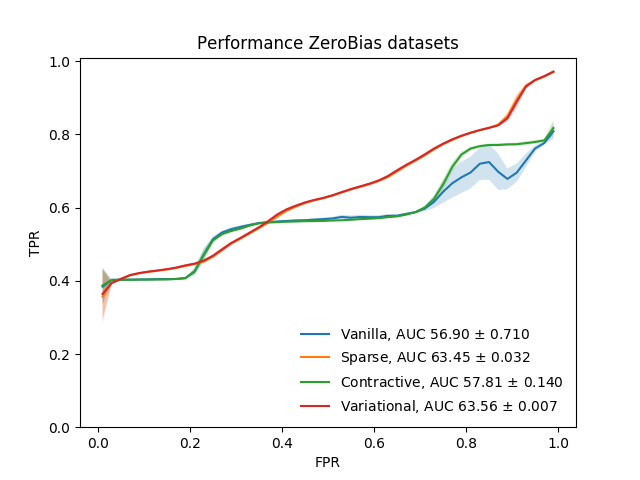
\includegraphics[width=\linewidth]{images/reco/2018/feature_2/performance_ZeroBias_VanillaSparseContractiveVariational.png}
        \caption{Zoom in}
    \end{subfigure}
    \begin{subfigure}[b]{0.49\linewidth}
        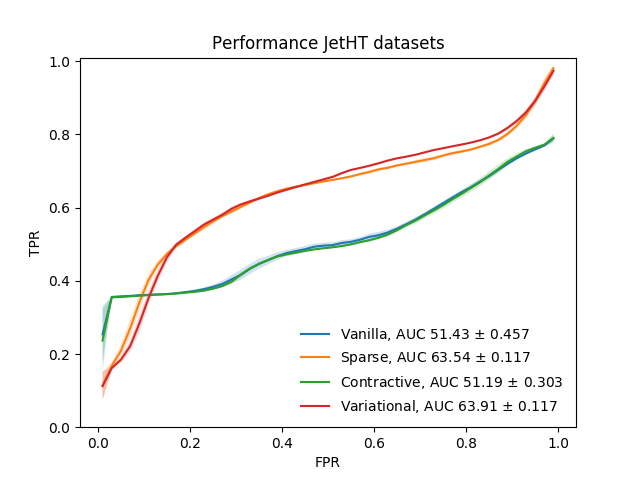
\includegraphics[width=\linewidth]{images/reco/2018/feature_2/performance_JetHT_VanillaSparseContractiveVariational.png}
        \caption{Full range}
    \end{subfigure}
    % \begin{subfigure}[b]{0.49\linewidth}
    %     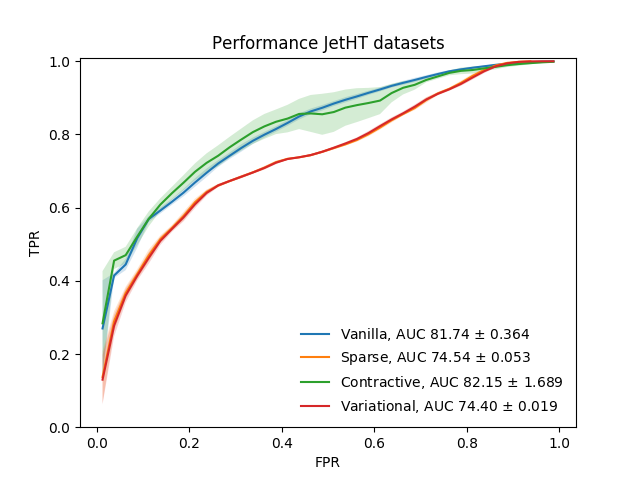
\includegraphics[width=\linewidth]{images/reco/2018/feature_1/performance_JetHT_VanillaSparseContractiveVariational.png}
    %     \caption{Zoom in}
    % \end{subfigure}
    \caption{Model performance for feature set 2 with 2018 data}
\label{fig:2018_f2_ae_performance}
\end{figure}

\begin{figure}[h!]
\centering
    \begin{subfigure}[b]{0.49\linewidth}
        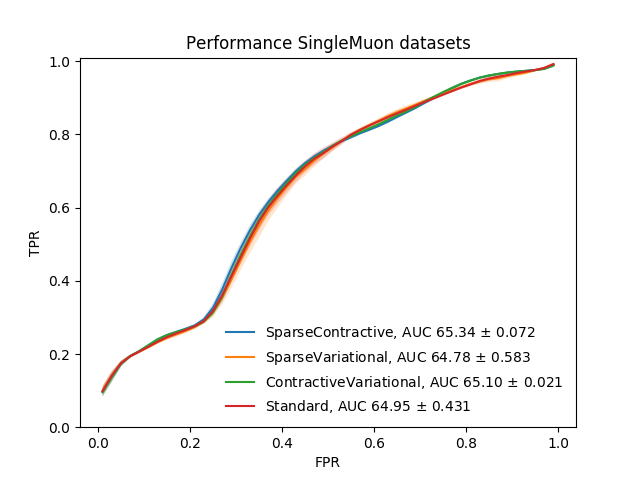
\includegraphics[width=\linewidth]{images/reco/2018/feature_2/performance_SingleMuon_SparseContractiveSparseVariationalContractiveVariationalStandard.png}
        \caption{Full range}
    \end{subfigure}
    \begin{subfigure}[b]{0.49\linewidth}
        \includegraphics[width=\linewidth]{images/reco/2018/feature_2/performance_ZeroBias_SparseContractiveSparseVariationalContractiveVariationalStandard.png}
        \caption{Zoom in}
    \end{subfigure}
    \begin{subfigure}[b]{0.49\linewidth}
        \includegraphics[width=\linewidth]{images/reco/2018/feature_2/performance_JetHT_SparseContractiveSparseVariationalContractiveVariationalStandard.png}
        \caption{Full range}
    \end{subfigure}
    % \begin{subfigure}[b]{0.49\linewidth}
    %     \includegraphics[width=\linewidth]{images/reco/2018/feature_1/performance_JetHT_VanillaSparseContractiveVariational.png}
    %     \caption{Zoom in}
    % \end{subfigure}
    \caption{Extended model performance for feature set 2 with 2018 data}
\label{fig:2018_f2_extended_ae_performance}
\end{figure}

\subsubsection{Distribution of decision value (to find the threshold)}
The distribution of decision value could be seen in Figure \ref{fig:2018_f2_se_dist}

\begin{figure}[h!]
\centering
    \begin{subfigure}[b]{0.49\linewidth}
        \includegraphics[width=\linewidth]{images/reco/2018/feature_2/se_dist_Vanilla1f2_SingleMuon_unlog.png}
        \caption{SingleMuon}
    \end{subfigure}
    \begin{subfigure}[b]{0.49\linewidth}
        \includegraphics[width=\linewidth]{images/reco/2018/feature_2/se_dist_Variational1f2_ZeroBias_unlog.png}
        \caption{ZeroBias}
    \end{subfigure}
    \begin{subfigure}[b]{0.49\linewidth}
        \includegraphics[width=\linewidth]{images/reco/2018/feature_2/se_dist_Variational1f2_JetHT_unlog.png}
        \caption{JetHT}
    \end{subfigure}
    \caption{Distribution of decision value}
\label{fig:2018_f2_se_dist}
\end{figure}

\subsubsection{Reconstruction Error}
Regarding Figure \ref{fig:2018_recon_error_singlemuon}, the peak around feature 50 in good LS is qglobTkN. Secondly, the couple clump around feature 80 is qglobTkChi2. The next pile is qglobTkNHits as well as last forky shape in around feature hundred dominated by qMuNCh. 

According to Figure \ref{fig:2018_recon_error_zerobias}, the residue in feature number 20 to 30 is qpVtxY. There are two huddles in bad LS where it mainly consists of qgTkPt, qgTkEta, and qgTkPhi. The clump in good LS around 70 to 80 mostly is qgTkPhi and qgTkN.

Lastly, by considering Figure \ref{fig:2018_recon_error_jetht}. Features that contain a very first peak in bad LS is qpVtxChi2. Secondly, around feature number 80 to 90 are qPFMetPt and qPFMetPhi. Lastly, there are the last two chunks of features (~120-127 and ~130-145) that behave like a noisy for both good and bad LS. Highly correlated features that show similar features (~15-35) are qpVtxX, qpVtxY, and qpVtxZ.

\begin{figure}[h!]
\centering
    \begin{subfigure}[b]{0.49\linewidth}
        \includegraphics[width=\linewidth]{images/reco/2018/feature_2/avg_sd_Vanilla_SingleMuon_f2_1.png}
        \caption{Sum over sampling}
    \end{subfigure}
    \begin{subfigure}[b]{0.49\linewidth}
        \includegraphics[width=\linewidth]{images/reco/2018/feature_2/sum_sd_Vanilla_SingleMuon_f2_1.png}
        \caption{Average over sampling}
    \end{subfigure}
    \caption{Reconstruction error of SingleMuon}
\label{fig:2018_recon_error_singlemuon}
\end{figure}

\begin{figure}[h!]
\centering
    \begin{subfigure}[b]{0.49\linewidth}
        \includegraphics[width=\linewidth]{images/reco/2018/feature_2/avg_sd_Variational_ZeroBias_f2_1.png}
        \caption{Sum over sampling}
    \end{subfigure}
    \begin{subfigure}[b]{0.49\linewidth}
        \includegraphics[width=\linewidth]{images/reco/2018/feature_2/sum_sd_Variational_ZeroBias_f2_1.png}
        \caption{Average over sampling}
    \end{subfigure}
    \caption{Reconstruction error of ZeroBias}
\label{fig:2018_recon_error_zerobias}
\end{figure}

\begin{figure}[h!]
\centering
    \begin{subfigure}[b]{0.49\linewidth}
        \includegraphics[width=\linewidth]{images/reco/2018/feature_2/avg_sd_Variational_JetHT_f2_1.png}
        \caption{Sum over sampling}
    \end{subfigure}
    \begin{subfigure}[b]{0.49\linewidth}
        \includegraphics[width=\linewidth]{images/reco/2018/feature_2/sum_sd_Variational_JetHT_f2_1.png}
        \caption{Average over sampling}
    \end{subfigure}
    \caption{Reconstruction error of JetHT}
\label{fig:2018_recon_error_jetht}
\end{figure}
\chapter{Conclusions}

\begin{itemize}
    \item Semi-supervised learning yields a remarkable result and well describe outlier LS
    \item So far, there is no grey zone from our model for this dataset
    \item Bad LS could be divided into two parts
    \begin{itemize}
        \item Bad with some pattern
        \item Anomaly
    \end{itemize}
\end{itemize}


% -------------------------------------------------------------------
% Bibliography
% -------------------------------------------------------------------

\bibliographystyle{agsm} 
\bibliography{mybibliography} 

% -------------------------------------------------------------------
% Appendices
% -------------------------------------------------------------------

% \begin{appendices}
% \chapter{An Appendix of Some Kind}

\lipsum[1-3]  % Replace with your text
% \chapter{Another Appendix}

\lipsum[1-3]  % Replace with your text

% \end{appendices}

\end{document}